\documentclass[11pt,letterpaper]{article}

\pagestyle{plain}                                    

\setlength{\textwidth}{6.5in}  
\setlength{\oddsidemargin}{0in}  
\setlength{\evensidemargin}{0in} 
\setlength{\textheight}{9in}    
\setlength{\topmargin}{0in}  
\setlength{\headheight}{0in}  
\setlength{\headsep}{0in}         
\setlength{\footskip}{.35in}       

\usepackage{amsmath}
\usepackage{natbib}
\usepackage{graphicx}
\usepackage{caption}
\usepackage{authblk}
\usepackage{float}
\usepackage{lineno}
\usepackage{rotating}
\usepackage{url}
\usepackage{placeins}
\linenumbers

\usepackage{titlesec}
\titleformat{\section}{\normalfont\fontsize{11}{11}\bfseries}{\thesection}{1em}{}
\titleformat{\subsection}{\normalfont\fontsize{11}{11}\bfseries}{\thesubsection}{1em}{}

\titlespacing\section{0pt}{11pt plus 2pt minus 2pt}{5.5pt plus 1pt minus 1pt}
\titlespacing\subsection{0pt}{11pt plus 2pt minus 2pt}{2pt plus 1pt minus 1pt}
\titlespacing\paragraph{0pt}{11pt plus 2pt minus 2pt}{2pt plus 1pt minus 1pt}

\begin{document}

\title{A Model to Calculate Fatigue Damage Caused by Partial Waking during Wind Farm Layout Optimization}

% \title{Wind Farm Layout Optimization with Constraints on Fatigue Caused by Partial Waking}
\date{}

\author[1]{Andrew P.J. Stanley}
\author[2]{Jennifer King}
\author[2]{Christopher Bay}
\author[1]{Andrew Ning}

\affil[1]{Department of Mechanical Engineering, Brigham Young University, Provo, UT, 84602, USA}

\affil[2]{National Renewable Energy Laboratory, National Wind Technology Center, Boulder, CO, 80303, USA}


\maketitle



\begin{abstract}
Wind turbines in wind farms often operate in waked or partially waked conditions, which can greatly increase the fatigue damage. Currently, the increased damage a turbine experiences in a wind farm is not considered in wind farm layout optimization because existing models are too computationally expensive. In this paper, we present a model to calculate fatigue damage caused by partial waking on a wind turbine which is computationally efficient and can be included in wind farm layout optimization. The model relies on analytic velocity, turbulence, and loads models commonly used in farm research and design, and captures some of the effects of turbulence on the fatigue loading. Compared to high fidelity simulation data, our model accurately predicts the damage trends of various waking conditions. We also perform example wind farm layout optimizations with our presented model in which we maximize the annual energy production of a wind farm while constraining the damage of the turbines in the farm. The results of our optimization show that the turbine damage can be significantly constrained with only a small sacrifice of around 1\% to the annual energy production.
\end{abstract}

Modern wind turbines are some of the largest machines in the world. Improvements in materials and technologies in recent years have allowed for taller towers, longer blades, and more power output \cite{wiser2016reducing,enevoldsen2019examining}. Because of their large size and associated large loads, as well as the cyclic loading caused by their rotational operation, fatigue is a vital consideration in wind turbine design \cite{hubler2019validation}. Turbines must be designed to operate without failure and with minimal maintenance for the duration of their lifetime, which is usually 20--25 years \cite{hu2016reliability,ziegler2018lifetime}. The cyclic load variations experienced by a wind turbine can be exacerbated when many turbines are built relatively close together in a wind farm. Wind turbines extract momentum from the moving air, creating a wake of slow moving wind behind them. In wind farms, turbine wakes can cause an uneven distribution of wind speeds across the swept rotor areas of downstream turbines, which intensifies the load fluctuations already present from turbulence and gravity. To make matters worse from a loads perspective, wind farms are usually optimized for maximum power production. Wind farm optimization can be used to refer to turbine layout optimization when constructing the farm, or active yaw control to steer wakes away from downstream turbines. In each case, the objective is typically to maximize power by reducing the velocity deficits caused by wakes. This optimization often leads to partially waked turbines which can be desirable for increasing power but devastating for the structure, causing turbines to fail earlier than expected and increasing overall costs. In order to account for increased fatigue damage caused by partial waking in wind farms, we developed a reduced order model to quickly calculate loads which can be used to constrain turbine damage in an optimization framework. 
% We optimized wind farms in a variety of scenarios to discover the effects that additional constraints for fatigue have on optimal wind farm design.

% Lit Review
Because they are large investments and their design is driven by fatigue, many researchers have studied how different conditions affect wind turbine loading and fatigue.
% 
An early study by Thomsen and S{\o}rensen used field data and the aeroelastic code HawC to examine how different atmospheric and waking conditions affect wind turbines. They found that fatigue loading increases by 5--15\% when a turbine is operating in a wake, compared to when it is operating in the freestream \cite{thomsen1999fatigue}.
% 
Another more recent paper by Meng et al.~finds similar results to the study performed by Thomsen and S{\o}rensen. They used the large eddy simulation code SOWFA and the finite element analysis code BECAS to find that, for an open-source reference turbine, the fatigue loads increased by 16\% when the turbine operated in a wake, compared to the freestream \cite{meng2019study}.
% 
A different paper by Kim et al.~found that when the turbulence intensity was increased from around 12\% to around 20\% in a wind farm, the fatigue loads increased between 30--50\% \cite{kim2015study}. This study highlights the importance of turbulence in calculating the fatigue on a wind turbine. All three of these studies indicate that loading and fatigue are greatly affected in wind farms, where waking and partial waking are normal operating conditions for many turbines in the farm.


In addition to characterizing fatigue loading in different conditions, several studies have been dedicated to using active control strategies to reduce fatigue loading on wind turbines. 
% 
In one of the first studies on using turbine control to reduce loads, Bossanyi showed that individual blade pitch control can be used to significantly reduce loading on the turbine structure \cite{bossanyi2003individual}.
% 
Njiri et al.~developed a control method in which the power production is slightly sacrificed to alleviate loads on the turbine structure. Near the end of a wind turbine's usual lifetime, the generator can be de-rated to extend it's lifetime. The bending moments on the blades can be reduced by more than 35\% by de-rating the generator from 100\% to 70\% \cite{njiri2019consideration}.
% 
Bernhammer et al.~performed a study with smart rotors, or rotors that use active aerodynamic devices (like flaps) to alter flow. They found that by using smart rotors, the loads can be reduced by 5--15\% \cite{bernhammer2016fatigue}.

% wind farm layout optimization
The studies mentioned above use active control of wind turbines themselves to reduce the loads experienced by wind turbines, with the implicit assumption that the inflow to the wind turbine cannot be controlled. 
% - However, the inflow to a wind turbine can be somewhat controlled  - I’d reword this.  Not really controlled.  More like the inflow can be changed if considered during the layout design phase.
However, the inflow can be changed if considered during the wind farm layout design phase.
With appropriate models, the loads experienced by each wind turbine in a farm can be predicted and constrained during optimization. 
Although this is a straightforward idea, current fatigue load prediction models are computationally expensive, and not suitable to be used in an optimization framework.
% 
% What We did
In this paper we present a model to quickly calculate load histories on wind turbine blades, and the associated fatigue damage. The presented model is fast enough to be used in a wind farm layout optimization, and predicts the damage trends for different waking and partial-waking conditions well compared to higher fidelity methods. 
% 
Additionally, we demonstrate the application of our newly presented model in example wind farm layout optimizations, and show how including fatigue damage constraints change the results of the optimization.

% Brief outline
% 
% 

\section{Wind Turbine Loads Model}
\label{sec1}
In this section, we describe the concepts and methods we used to estimate the loads and fatigue damage at the blade root of a wind turbine, and how the various steps and models fit together. 
% 
Before discussing the specifics of our methodology, it is important that we mention a few items. 
First, our proposed method relies on the ability to calculate the velocities and local turbulence intensities at various points throughout the wind farm. 
% Less accurate wind farm wake models and turbulence intensity estimates will be able to predict the correct trends, but will not be as successful in predicting the actual load histories and damage values. 
We will discuss the models that we used and found success with. 
Second, we have validated our various models with the large eddy simulation software Simulator fOr Wind Farm Applications (SOWFA) \cite{churchfield2012nwtc}, and the aeroelastic structural analysis software OpenFAST \cite{openfast_docs}. Both of these programs are open-source, and created at the National Renewable Energy Laboratory (NREL). We used the velocity data from SOWFA as the velocity input into OpenFAST to calculate the load histories on a wind turbine for various waking conditions. For the models and results shown in this paper we used the NREL 5-MW reference turbine, which is an open-source turbine design used in many research studies \cite{jonkman2009definition}.
Refer to Appendix 1 for more details about our SOWFA simulations.

The rest of this section will discuss the various details of the loads and damage model that we present in this paper. 
Fatigue damage on a wind turbine is caused by cyclic loading as a turbine rotates. These load variations are caused by gravity, uneven wind speeds across the rotor caused by partial waking, and turbulence. In fact, the loads on a turbine are more complicated than this, because they depend on the interactions of all of these causes.
To account for the interactions of all of these fatigue drivers, our model predicts the loads on a turbine blade at a predetermined number of azimuth angles and blade rotations. The predicted load history is then used to calculate the fatigue damage a turbine blade experiences for a given turbine layout and wind condition.
Figure \ref{flow-chart} shows a general overview the model. As each part of the model is important and has some subtleties, each will be discussed individually.
% 
\begin{figure}
    \centering
    \includegraphics[]{images/fatigue-model_up.pdf}
    \caption{A flow chart of the damage calculation model used in this study.}
    \label{flow-chart}
\end{figure}

\subsection{Generate Turbulence Samples}

% The first step is to sample from a turbulence distribution. 
% To account for the effect turbulence has on the loads, we scaled the steady state loads at the desired azimuth angles and for the selected number of rotations with the turbulence. Thus, the total number of turbulence samples required was the number of desired azimuth angles multiplied by the number of rotations to be modeled. 
% The results shown in this paper are for two azimuth angles, 90 and 270 degrees. These angles are when the blades are parallel to the ground on each side of the rotor, and represent the extremes of the load cycles caused by gravity and by partial waking. In addition, we modeled 100 full rotations of the rotor, meaning that we needed 200 turbulence samples.
% We assumed that the velocity variations due to turbulence were Gaussian and used Latin hypercube sampling to sample from a normal distribution with a mean of zero and a standard deviation of one.  

% In addition to the values sampled, the order in which they appear is important. The model performs best when the distribution formed by taking the difference of sequential values is also approximately Gaussian. With a large enough sample, a random sample of a normal distribution will automatically meet this criterion. However, there is no guarantee for smaller samples. Thus, it is important to check that the samples and the difference of sequential values of the samples are approximately Gaussian. In this paper, we evaluated the loads at two azimuth angles for one hundred blade rotations, meaning we needed two hundred turbulence samples. The distribution we used is shown in in the left subfigure of Fig.~\ref{samples}, and the distribution formed by the difference between sequential values of the samples is shown in the right subfigure.
% 
% \begin{figure}
%     \centering
%     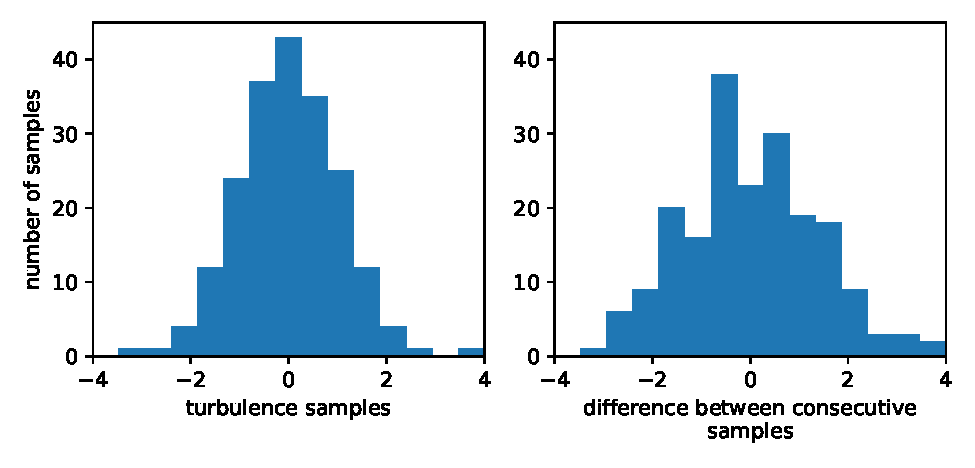
\includegraphics[]{images/turbulence_samples.pdf}
%     \caption{Histogram of the turbulence samples taken for this study. On the left are the 100 turbulence samples, on the right is the distribution formed by the difference of sequential values from the turbulence samples.}
%     \label{samples}
% \end{figure}

One large driver of fatigue damage in a wind turbine is turbulence. The severity of turbulence is usually described with turbulence intensity, which is a measure of the standard deviation of the wind speed divided by its mean. This provides a time averaged description of the turbulence, but provides no information about the instantaneous values. In order to account for the instantaneous values, we created a set of turbulence samples $S$, which is some set of values with a standard deviation of one and mean value of zero. These samples are scaled later by the local turbulence intensity and the mean wind speed to obtain instantaneous velocities and loads. 

There are a variety of possible methods that could be used to define these turbulence samples. We tried two different methods. The first was to assume that the velocity variations due to turbulence were Gaussian, and used Latin hypercube sampling to sample from a normal distribution with a mean of zero and a standard deviation of one. We then shuffled the samples such that the difference of sequential values in the distribution was also approximately Gaussian. This was important because the fatigue damage depends on the order in which loads appear. The second method we tried was to use the turbulence generator TurbSim to generate the turbulence samples \cite{jonkman2006turbsim}. This creates a more realistic turbulence history, but requires using an external program. For the results shown in this paper, the turbulence history was generated by TurbSim, an example of which is shown in Fig.~\ref{turb_samps}.

\begin{figure}
    \centering
    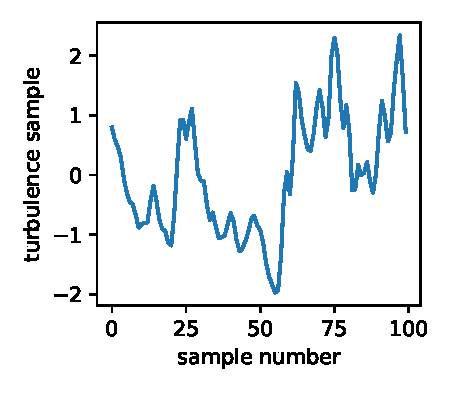
\includegraphics[]{images/turb_samps.pdf}
    \caption{An example set of turbulence samples taken for this study.}
    \label{turb_samps}
\end{figure}

% The first step is to sample from a turbulence distribution. 
% To account for the effect turbulence has on the loads, we scaled the steady state loads at the desired azimuth angles and for the selected number of rotations with the turbulence. Thus, the total number of turbulence samples required was the number of desired azimuth angles multiplied by the number of rotations to be modeled. 
% There are several methods that could be used to obtain the turbulence samples. 



\subsection{Calculate Steady-State Effective Turbine Wind Speed}

After defining the turbulence samples, the next step is to calculate the steady-state effective turbine wind speed. This is done with an analytic wake model used to predict wind speeds in a wind farm. For this paper, we found good results with a modified Gaussian wake model presented by Bastankhah and Porté-Agel \cite{bastankhah2016experimental}.
% 
The original formulation of the model does not define the wake deficit in the near wake region. This near-wake region, called the potential core, results in regions behind wind turbines where the wind speed is undefined. These undefined regions in the space make optimization difficult, as the objective function is undefined is some places. To mitigate this issue, Thomas and Ning added a linear interpolation of the wake loss from the turbine up to where it is defined by the wake model, which is the version used in this paper \cite{Thomas2018}. 
The most important equation for this Gaussian wake model is shown in Eq.~\ref{wake-model}:
% 
\begin{equation}
    \label{wake-model}
    \frac{\Delta\bar{u}}{\bar{u}_{\infty}} = \Bigg(1 - \sqrt{1 - \frac{C_T \cos{\gamma}}{8\sigma_y\sigma_z/d^2}}  \Bigg) \exp{\bigg(-0.5\Big(\frac{y-\delta}{\sigma_y} \Big)^2}\bigg) \exp{\bigg(-0.5\Big(\frac{z-z_h}{\sigma_z} \Big)^2}\bigg)
\end{equation}
%
\noindent where $\Delta\bar{u}/\bar{u}_{\infty}$ is the velocity deficit in the wake; $C_T$ is the thrust coefficient; $\gamma$ is the yaw angle, which is assumed to be zero throughout this paper; $y-\delta$ and $z-z_h$ are the distances from the wake center and the point of interest in the cross-stream horizontal and vertical directions, respectively; and $\sigma_y$ and $\sigma_z$ are the standard deviations of the wake deficit, again in the cross-stream horizontal and vertical directions, respectively. These standard deviations are defined in Eqs.~\ref{sigma_y} and \ref{sigma_z}.
%
\begin{equation}
    \label{sigma_y}
    \sigma_y = k_y(x-x_0) + \frac{D\cos{\gamma}}{\sqrt{8}}
\end{equation}
%
\begin{equation}
    \label{sigma_z}
    \sigma_z = k_z(x-x_0) + \frac{D}{\sqrt{8}}
\end{equation}
%
\noindent where $D$ is the diameter of the wind turbine creating the wake, $x-x_0$ is the distance downstream from the end of the potential core to the point of interest, and $k_y$ and $k_z$ are unitless, and are functions of the freestream turbulence intensity:
%
\begin{equation}
    \label{turbulence}
    k_y,k_z = a\text{TI}+b
\end{equation}
%
In Eq.~\ref{turbulence}, $a$ and $b$ are tuning parameters, while $\text{TI}$ is the effective turbulence intensity to the upstream wind turbine. 
% For this paper, we used the tuning parameters $a=0.4062$ and $b=0$. 
The length of the potential core, $x_0$ is defined in Eq.~\ref{potential_core}.
%
\begin{equation}
    \label{potential_core}
    x_0 = \frac{D \cos{\gamma} (1 + \sqrt{1-C_T})}{\sqrt{2}[\alpha^*\text{TI} + \beta^* (1-\sqrt{1-C_T})]}
\end{equation}
% 
In this equation, $\alpha^*$ and $\beta^*$ are turning parameters.
% , for which we used the values $\alpha^*=8.059$ and $\beta^*=0$ in this paper. 
With the correct tuning parameters, we were able to approximate velocity data from SOWFA with the analytic wake model. 
% 
Note that because the yaw angle, $\gamma$, is assumed to be zero throughout this paper, $\cos(\gamma)=1$ meaning that $\sigma_y=\sigma_z$. 

To calculate the the loads on a wind turbine in this study, we needed to be able to accurately predict the local turbulence intensity throughout the wind farm. Additionally, for this wake model we need the effective turbulence intensity for the inflow into a turbine. We used two different models to fit these two requirements. The model to calculate local turbulence intensity will be discussed in Section \ref{sec:TI}, while the algorithm to calculate the effective inflow turbulence intensity to a turbine is given in Thomas et al.~\cite{Thomas2019}.


Figures \ref{vels_lowTI} and \ref{vels_highTI} show the velocity profiles predicted by the wake model compared to the time average velocity data from our SOWFA runs for 4, 7, and 10 diameters downstream of a wind turbine. Each figure shows a horizontal sweep across the wake at hub height, at the distance downstream that is indicated. Note that the model has been tuned for each wind speed and turbulence intensity. For the low turbulence intensity cases, there is good agreement between the model and the SOWFA data for every wind speed. For the higher turbulence intensity cases shown in Fig.~\ref{vels_highTI}, the model does a decent job at predicting the wind speeds, however the comparison is not as good as that with the low turbulence. The model does not capture the asymmetry in the wake, or any local velocity differences in the freestream. Notice that with low turbulence, the wakes propagate farther, leading to larger velocity deficits downstream of the turbine. With higher turbulence, the wakes dissipate more quickly leading to smaller velocity deficits. 
% 
% \begin{figure}
%     \centering
%     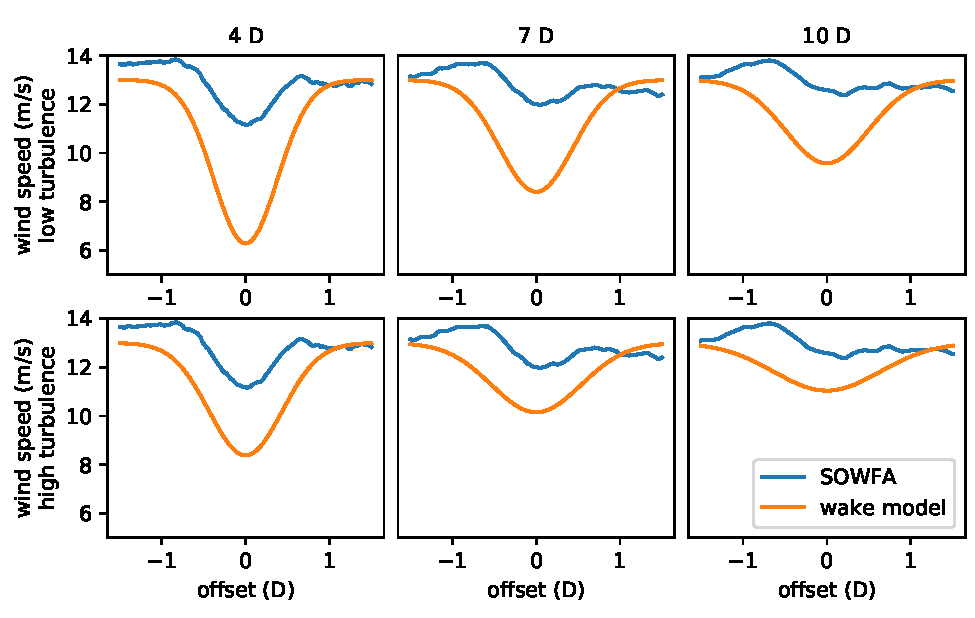
\includegraphics[]{images/velocity_profiles.pdf}
%     \caption{The wake deficits predicted by our large eddy simulation data compared to our analytic wake model. The row on the top is for a low turbulence intensity of 4.6\%, while the bottom is for a high turbulence intensity of 8\%. From left to right, each column represents the wake deficits at 4, 7, and 10 rotor diameters downstream of the turbine generating the wake.}
%     \label{velocity_profiles}
% \end{figure}
% 
\begin{figure}
    \centering
    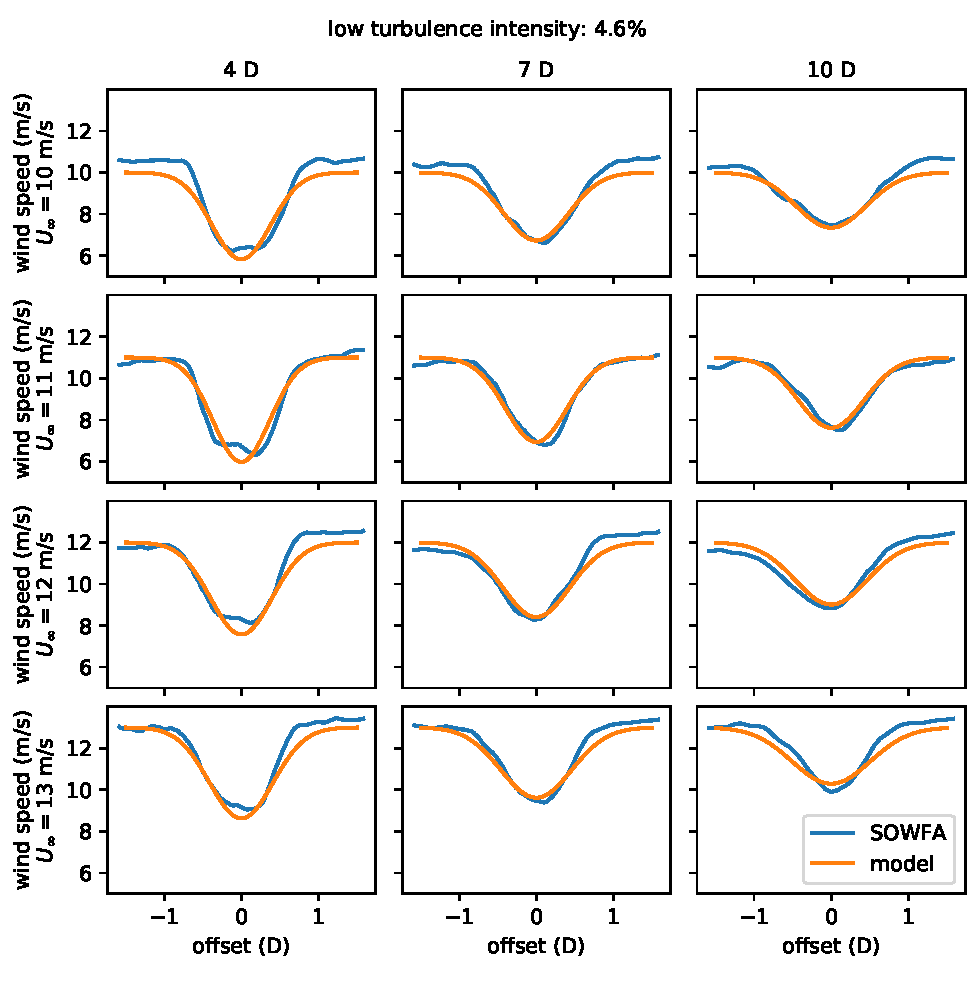
\includegraphics[]{images/vels_lowTI.pdf}
    \caption{The wake deficits predicted by our large eddy simulation data compared to our analytic wake model for a lower turbulence intensity of 4.6\%. From left to right, each column represents the wake deficits at 4, 7, and 10 rotor diameters downstream of the turbine generating the wake. From top to bottom, each row represents the wake deficits with a freestream wind speed of 10, 11, 12, and 13 m/s.}
    \label{vels_lowTI}
\end{figure}
% 
\begin{figure}
    \centering
    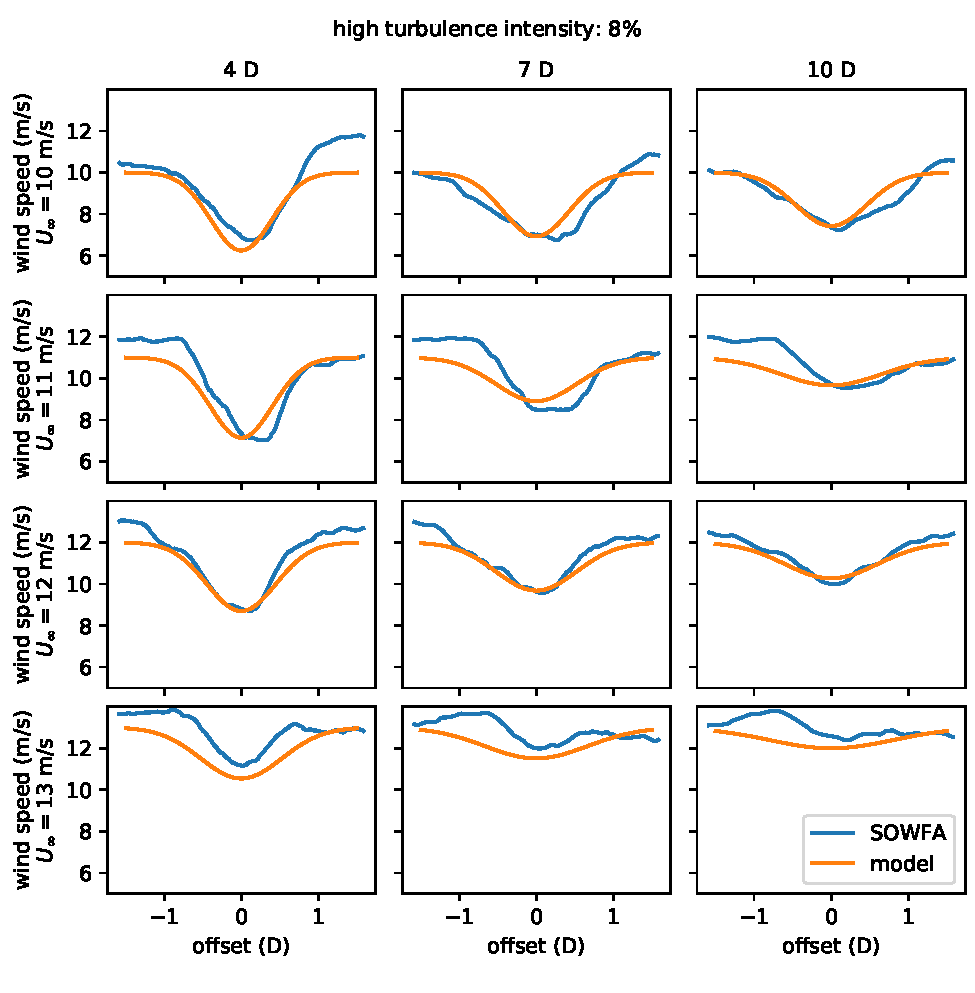
\includegraphics[]{images/vels_highTI.pdf}
    \caption{The wake deficits predicted by our large eddy simulation data compared to our analytic wake model for a higher turbulence intensity of 8\%. From left to right, each column represents the wake deficits at 4, 7, and 10 rotor diameters downstream of the turbine generating the wake. From top to bottom, each row represents the wake deficits with a freestream wind speed of 10, 11, 12, and 13 m/s.}
    \label{vels_highTI}
\end{figure}

In the case of combined wakes, the total wind speed was calculated with a linear combination method, represented in Eq.~\ref{combination}.
%
\begin{equation}
    \label{combination}
    \bar{u} = \bar{u}_\infty - \sum_{i=1}^\text{nTurbs} u_i \Big(\frac{\Delta\bar{u}}{\bar{u}_{\infty}}\Big)_i
\end{equation}
% 
In this equation, $\bar{u}$ is the local wind speed at a given point, $\bar{u}_\infty$ is the freestream wind speed, $\text{nTurbs}$ is the number of wind turbines upstream of the point of interest, $u_i$ is the inflow speed of an upstream turbine, and $\Big(\frac{\Delta\bar{u}}{\bar{u}_{\infty}}\Big)_i$ is the velocity deficit from an upstream turbine. This wake combination method has been shown to work well with the Gaussian wake model we used \cite{niayifar2016analytical}.

The wake model above has all been defined to calculate the wind speed at a given point. To determine the effective wind speed into a wind turbine, we took the average of the wind speed calculated at four points across the rotor, shown in Fig.~\ref{speed_samples}. We have found that sampling at these four points gives an almost identical effective wind speed as sampling with many more points across the rotor.
% 
\begin{figure}
    \centering
    \hspace*{0.7cm} 
    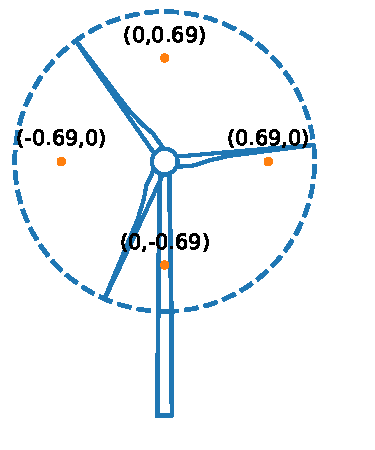
\includegraphics[]{images/rotor_samples_1.pdf}
    \caption{The sample points used to calculate the effective wind speed into a turbine.}
    \label{speed_samples}
\end{figure}

This section has discussed in detail the analytic wake model we used in this paper. Remember that the fatigue model that we will present does not require this specific wake model. However, it does depend on the ability to provide accurate wind speeds for various locations throughout the wind farm. We have found success with the wake model presented in this section, however other wake models or methods to calculate the wind speed may also be used, as far as they are accurate. 

\subsection{Calculate Effective Blade Turbulence Intensity}
\label{sec:TI}

The next step in the model is to calculate the effective blade turbulence intensity at each azimuth angle, which is defined as the standard deviation of the streamwise wind speed divided by the mean. This requires the ability to accurately calculate the turbulence intensity at any given location. To accomplish this, we used a modified version of the model presented by Ishihara and Qian \cite{ishihara2018new}. This turbulence intensity model is shown in Eq.~\ref{ti_eq}.
%
\begin{equation}
    \label{ti_eq}
    \Delta \text{TI}(x,y,z) = \frac{1}{d + e \cdot x/D + f\cdot(1+x/D)^{-2}} \cdot \Big\{k_1 \exp{-\frac{(r-D/2)^2}{2\sigma_t^2}} + k_2 \exp{-\frac{(r+D/2)^2}{2\sigma_t^2}} \Big\} - \delta(z)
\end{equation}
% 
In this equation, $\text{TI}$ is the added turbulence intensity caused by an upstream wind turbine, $x$ and $y$ are the downstream and cross-stream distances from the point of interest to the upstream turbine, $z$ is the height of the point of interest, and $D$ is the rotor diameter of the upstream turbine. The rest of the values are represented by the following equations. The values for $d$, $e$, and $f$ are given by Eqs.~\ref{d_val}, \ref{e_val}, and \ref{f_val}.
%
\begin{equation}
    \label{d_val}
    d = 2.3C_T^{-1.2}
\end{equation}
%
\begin{equation}
    \label{e_val}
    e = \text{TI}_a^{0.1}
\end{equation}
%
\begin{equation}
    \label{f_val}
    f = 0.7C_T^{-3.2} \text{TI}_a^{-0.45}
\end{equation}
In these equations, $C_T$ is the thrust coefficient of the upstream wind turbine, and $\text{TI}_a$ is the ambient turbulence intensity. The radial distance to the point of interest, $r$ , is given by Eq.~\ref{r_val},
%
\begin{equation}
    \label{r_val}
    r = \sqrt{y^2 + (z-H)^2}
\end{equation}
where $H$ is the hub height of the upstream turbine. The values for $k_1$ and $k_2$ are given in Eqs.~\ref{k1_val} and \ref{k2_val}.
%
\begin{equation}
    \label{k1_val}
    k_1 = \begin{cases} 
      \cos^2{(\pi/2 \cdot (r/D - 0.5))} & r/D \leq 0.5 \\
      1 & r/D > 0.5
   \end{cases}
\end{equation}
%
\begin{equation}
    \label{k2_val}
    k_2 = \begin{cases} 
      \cos^2{(\pi/2 \cdot (r/D + 0.5))} & r/D \leq 0.5 \\
      0 & r/D > 0.5
   \end{cases}
\end{equation}
% 
Finally, $\sigma_t$ is a representative wake width for the local turbulence intensity model, which is shown in Eq.~\ref{sigma_val}.
%
\begin{equation}
    \label{sigma_val}
    \sigma_t/D = k^* x/D + \epsilon
\end{equation}
% 
The values for $k^*$ and $\epsilon$ are given in Eqs.~\ref{k_val} and \ref{eps_val}.
%
\begin{equation}
    \label{k_val}
    k^* = 0.11 C_T^{1.07} \text{TI}_a ^ {0.20}
\end{equation}
%
\begin{equation}
    \label{eps_val}
    \epsilon = 0.23 C_T^{-0.25} \text{TI}_a^{0.17}
\end{equation}

We made some slight adjustments to this model by introducing two tuning parameters $C_1$ and $C_2$, which change Eqs.~\ref{ti_eq} and \ref{sigma_val}. The new equations are shown in Eqs.~\ref{new_ti} and \ref{new_sig}.
% 
\begin{equation}
    \label{new_ti}
    \Delta \text{TI}(x,y,z) = \frac{1}{C_1}(\frac{1}{d + e \cdot x/D + f\cdot(1+x/D)^{-2}} \cdot \Big\{k_1 \exp{-\frac{(r-D/2)^2}{2\sigma_t^2}} + k_2 \exp{-\frac{(r+D/2)^2}{2\sigma_t^2}} \Big\} - \delta(z))
\end{equation}
%
\begin{equation}
    \label{new_sig}
    \sigma_t/D = \frac{1}{C_2}(k^* x/D + \epsilon)
\end{equation}

Figures \ref{TI_lowTI} and \ref{TI_highTI} show the predicted turbulence intensity from the model compared to our SOWFA data. Each of the figures show a sweep across the turbine wake at hub height. Figure \ref{TI_lowTI} shows the model comparison for a low freestream turbulence of 4.6\%. There is good comparison between the analytic model, representing the trends and actual values of the local turbulence intensities. Figure \ref{TI_highTI} shows the model comparison for a high freestream turbulence of 8\%. With high freestream turbulence, the analytic model does not match the SOWFA data as well. The local turbulence intensity does not follow the same structure as the model predicts. As with the wake model shown in the previous section, the turbulence intensity model represented in these figures has been tuned for each freestream wind speed and turbulence intensity.
% % 
% \begin{figure}
%     \centering
%     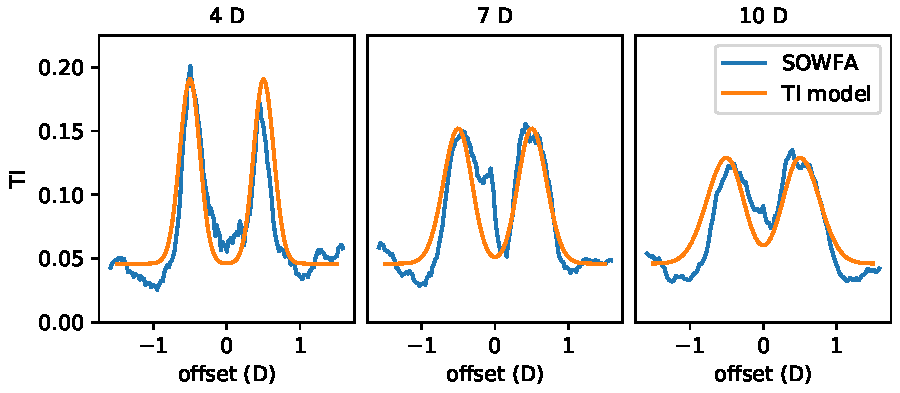
\includegraphics{images/turbulence_profiles.pdf}
%     \caption{The turbulence intensity predicted by our large eddy simulation data compared to our analytic turbulence intensity model. This figure is for a freestream turbulence of 4.6\%. From left to right, each subfigure represents the turbulence intensity at 4, 7, and 10 rotor diameters downstream of the turbine shedding the wake.}
%     \label{turbulence_sweep}
% \end{figure}
% 
\begin{figure}
    \centering
    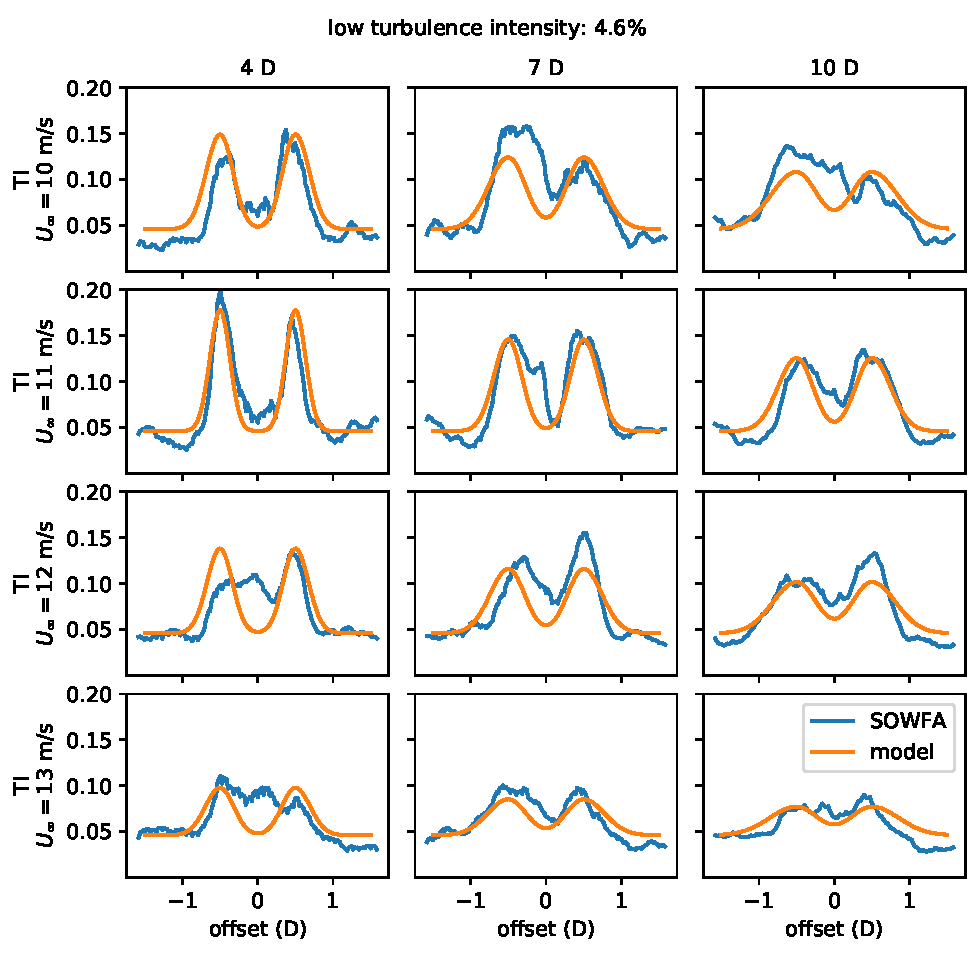
\includegraphics{images/TI_lowTI.pdf}
    \caption{The turbulence intensity predicted by our large eddy simulation data compared to the analytic turbulence intensity model for a lower freestream turbulence intensity of 4.6\%. From left to right, each column represents the turbulence intensities at 4, 7, and 10 rotor diameters downstream of the turbine generating the wake. From top to bottom, each row represents the turbulence intensities with a freestream wind speed of 10, 11, 12, and 13 m/s.}
    \label{TI_lowTI}
\end{figure}
% 
\begin{figure}
    \centering
    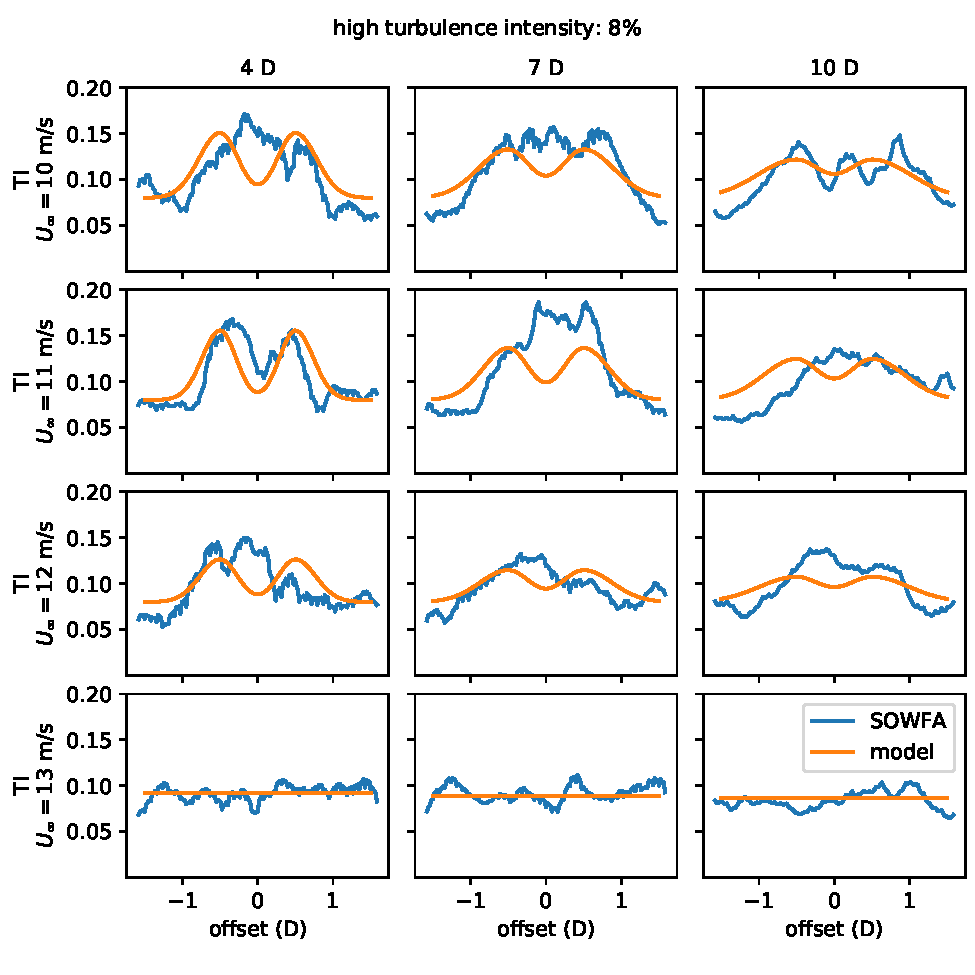
\includegraphics{images/TI_highTI.pdf}
    \caption{The turbulence intensity predicted by our large eddy simulation data compared to the analytic turbulence intensity model for a higher freestream turbulence intensity of 8\%. From left to right, each column represents the turbulence intensities at 4, 7, and 10 rotor diameters downstream of the turbine generating the wake. From top to bottom, each row represents the turbulence intensities with a freestream wind speed of 10, 11, 12, and 13 m/s.}
    \label{TI_highTI}
\end{figure}

With the turbulence intensity model defined, the effective turbulence intensity over the entire blade can be calculated. This is done by integrating the turbulence intensity over the length of the blade, as shown in Eq.~\ref{int_ti}.
%
\begin{equation}
    \label{int_ti}
    \text{TI}_{\text{eff}} = \frac{1}{R_{\text{tip}}}\int_0^{R_\text{tip}} \text{TI}(r)~dr
\end{equation}
%
In this equation, $\text{TI}_{\text{eff}}$ is the effective turbulence intensity over the length of the blade, $R_{\text{tip}}$ is the radius of the blade at the tip, $\text{TI}$ is the local turbulence intensity evaluated along the length of the blade, $r$. This effective turbulence intensity for the blade is evaluated for each azimuth angle that is being considered.

In addition to the turbulence intensity for the blade, we also calculate an effective turbulence intensity for the entire rotor, $\text{TI}_{\text{eff, rotor}}$. This is defined as the average of the effective blade turbulence intensities calculated at each azimuth angle.

\subsection{Calculate Steady-State Bending Moments}

The next step in this model is to calculate the steady state bending moments on the blade at each azimuth angle of interest. First, the loading across the blade must be calculated with the wind speeds that vary across the blade, using the same wake model described in step 2. We calculated the loads using CCBlade, a blade element momentum method for propellers and turbines \cite{Ning2020}. In addition to the wind speeds experienced across the blade, these loads are dependent on the rotor rotation speed and the blade pitch angle. These values are determined with the turbine control scheme and the effective turbine inflow speed calculated in step 2. The rotation speed is determined from the ideal tip-speed ratio of the wind turbine, shown in Eq.~\ref{omega_tsr}. 
% 
\begin{equation}
    \Omega = \begin{cases} 
      \lambda U_\text{eff}/R &  U_\text{eff} \leq U_\text{rated} \\
      \Omega_\text{rated} &  U_\text{eff} > U_\text{rated}\\
   \end{cases}
   \label{omega_tsr}
\end{equation}
% 
In this equation, $\Omega$ is the rotation speed, $\lambda$ is the tip-speed ratio from the turbine definition, $U_\text{eff}$ is the effective turbine inflow speed, $R$ is the rotor radius, $U_\text{rated}$ is the rated turbine wind speed, and $\Omega_\text{rated}$ is the rated turbine rotation speed.
The pitch angle is also a function of inflow wind speed, and depends on the control scheme that is used. The pitch angles for the NREL 5-MW reference turbine are shown in Fig.~\ref{pitch_fig}. Note that we applied a slight smoothing to the pitch function at the rated wind speed to facilitate optimization.
% 
\begin{figure}
    \centering
    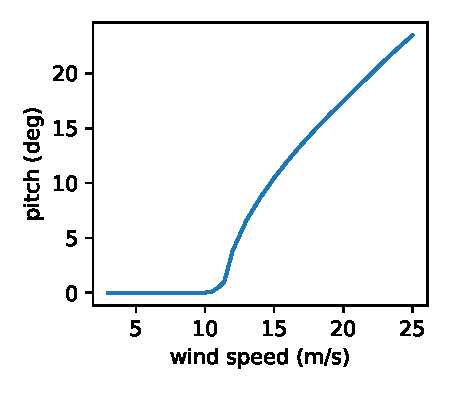
\includegraphics[]{images/pitch_degs.pdf}
    \caption{Blade pitch angle versus wind speed for the NREL 5-MW reference turbine.}
    \label{pitch_fig}
\end{figure}

After calculating the loads along the blade, the moments can be determined by integrating the loads along the length of the blade, show in Eq.~\ref{int_moms}. 
%
\begin{equation}
    \label{int_moms}
    M = \int_0^{R_{\text{tip}}} Fr~dr
\end{equation}
%
In this equation, $M$ is the bending moment caused by the loading along the blade, $F$ is the loading along the blade, and $r$ is the distance along the blade.
This is done for both the flapwise and lead-lag loads along the turbine blade. Because CCBlade only returns the aerodynamic loading on the blade, it is important to also add on the moment caused by gravity to the lead-lag moment.

In the results for this paper, we have assumed that the fatigue critical area is at the blade root, where the bending moments are the highest. Although this may not always be the case, it is a safe assumption to demonstrate the methodology and functionality of our model.

\subsection{Turbulence and Azimuth Loop}

The three sections following this one discuss steps 6, 7, and 8. These steps occur in a loop, which creates a load history which accounts for the different azimuth angles of the blade, and the different loading that occurs at each rotation caused by turbulence. 
For all the cases that we tested, two azimuth angles of 90 degrees and 270 degrees are sufficient to predict the fatigue damage. These azimuth angles correspond to when the turbine blade is parallel to the ground on opposite sides of the rotor. At these angles, the gravitational loading is at the extreme values. Additionally, the load variations caused by partial waking are the largest between these two azimuth angles. In some cases with high wind shear, it may be appropriate to also include azimuth angles of 0 and 180 degrees, between which the differences in wind speed due to wind shear are the largest. However, at these angles the moments due to gravity are zero, indicating that the flapwise loads would need to be very large to introduce larger load fluctuations than would occur at azimuth angles of 90 and 270 degrees. Therefore, for most conditions just considering these two azimuth angles is sufficient. %In addition to these two azimuth angles, for this paper we create our loads distribution with 100 full blade rotations. We found that this was sufficient to converge the damage values within an acceptable tolerance, while still maintaining the desired fast computational speed.

\subsection{Calculate Turbulent Effective Turbine Wind Speed}

Once in the loop, the first step is to calculate the effective turbine wind speed with turbulence. Turbulence intensity at a given point is defined in Eq.~\ref{turb_intensity}.
%
\begin{equation}
    \label{turb_intensity}
    \text{TI} = \frac{\sigma_u}{\bar{u}}
\end{equation}
% 
In this equation, $\sigma_u$ is the standard deviation of the streamwise wind speed, and $\bar{u}$ is the mean wind speed at the given point. Using this definition of turbulence intensity, we defined the instantaneous effective turbine velocity in Eq.~\ref{turbulent_inflow}.
%
\begin{equation}
    \label{turbulent_inflow}
    U_{\text{turbulent}} = U_{\text{steady}}(1 + S_i ~\text{TI}_{\text{eff, rotor}})
\end{equation}
% 
In this equation, $U_{\text{turbulent}}$ is the instantaneous effective turbine inflow which accounts for turbulence, $U_{\text{steady}}$ is the steady state turbine inflow velocity calculated in step 2, and $S_i$ is the turbulence sample corresponding to the azimuth angle and rotation being calculated, which was defined in step 1. The turbulence intensity $\text{TI}_{\text{eff, rotor}}$ is the effective rotor value calculated in step 3. 

\subsection{Calculate Rotational Speed and Pitch Angle}
% This step is very simple, but is important when calculating the damage later on. 
Using the control scheme of the turbine being modeled, the rotational speed of the turbine is calculated and stored based on the turbulent effective turbine wind speed calculated previously. The instantaneous pitch angle is also calculated, which will be used when finding the instantaneous bending moments.


\subsection{Calculate Turbulent Bending Moments}
This next critical step is to calculate the bending moment history with the instantaneous wind speeds that take turbulence into account. This could be done directly, by calling CCBlade within the turbulence and azimuth angle loop to get the blade loads, then convert them into bending moments. However, this is unnecessarily expensive. Sufficiently accurate bending moments can be calculated by simply adjusting the steady bending moment calculated in step 4 based on the turbulence. The bending moments scale as a function of the wind speed and the pitch angle. These relationships can be determined from the specific blade design for the turbine of interest using CCBlade, and calculating the moments for different wind speeds and pitches angles. For example, for the NREL 5-MW reference turbine blades, we determined that the moments scaled exponentially with increasing wind speed. This was obtained by performing a least squares fit to the moments as a function of the wind speed. The relation is shown in Eq.~\ref{scale_speed}.
% 
\begin{equation}
    M_\text{turb} = M_{\text{steady}}*\Big(\frac{U_\text{turb}}{U_\text{steady}}\Big)^e
    \label{scale_speed}
\end{equation}
% 
In this equation, $M_\text{turb}$ is the instantaneous bending moment accounting for turbulence, $M_{\text{steady}}$ is the steady state bending moment calculated in step 4, $U_\text{turb}$ is the instantaneous turbulent wind speed, and ${U_\text{steady}}$ is the steady state wind speed. The exponent, $e$, was determined to be 1.285 to best represent the turbine blades. The instantaneous turbulent wind speed is calculated using the turbulence samples created in step 1, the effective blade turbulence intensity for the azimuth angle of interest calculated in step 3, and the steady wind speed, as shown in Eq.~\ref{turb_speed}.
% 
\begin{equation}
    U_\text{turb} = U_\text{steady} + U_\text{steady} S_i \text{TI}_{\text{eff}}
    \label{turb_speed}
\end{equation}
% 
In this equation, $\text{TI}_{\text{eff}}$ is the effective blade turbulence intensity, and $S_i$ is the instantaneous turbulence sample. Equation \ref{turb_speed} can then be substituted into Eq.~\ref{scale_speed}, resulting in Eq.~\ref{scale_turb}.
% 
\begin{equation}
    M_\text{turb} = M_{\text{steady}} (1+ S_i \text{TI}_{\text{eff}})^e
    \label{scale_turb}
\end{equation}
% 
% (1.0 + turb_samples[i]*TI_inst)
%, with the exponent of 1.285. 
Similarly, the loads as a function of the pitch angle are determined. For the reference blade used in this study, we found that the effect pitch angle has on loads could be approximated linearly for the flapwise moments, and quadratically for the lead-lag moments. The relations used to calculate the turbulent blade bending moments as a function of pitch angles are shown in Eqs.~\ref{pitch_flap} and \ref{pitch_edge}.
% 
\begin{equation}
    M_\text{flap,pitched} = M_{\text{flap,turb}} - m~ \theta_{\text{diff}}
    \label{pitch_flap}
\end{equation}
% 
\begin{equation}
    M_\text{ll,pitched} = M_{\text{ll,turb}} - ((\theta_{\text{diff}} - p)~q)^2
    \label{pitch_edge}
\end{equation}
In these equations, $M_\text{flap,pitched}$ and $M_\text{ll,pitched}$ are the flapwise and lead-lag bending moments which take additional pitch into account, $M_{\text{flap,turb}}$ and $M_{\text{ll,turb}}$ are the scaled, turbulent bending moments, $\theta_{\text{diff}}$ is the difference between the instantaneous pitch angle calculated in step 7, and the steady-state pitch angle in radians. The other variables $m=47{,}275$, $p=0.5$, and $q=280$ represent constants that are specific to the turbine blade used, which we determined using least squares regression to moments calculated with CCBlade.
% edge[i] = aero_edge - ((pitch_diff-m)*n)^2

% This adjustment is shown in Eq.~\ref{adjust_moms}.
% % 
% \begin{equation}
%     \label{adjust_moms}
%     M_{\text{turbulent}} = M_{\text{steady}}(1 + S_i ~\text{TI}_\text{eff})
% \end{equation}
% % 
% As in Eq.~\ref{turbulent_inflow}, $S_i$ is the turbulence sample for the azimuth angle and cycle being computed. The moment $M_{\text{turbulent}}$ is the bending moment considering turbulence, while $M_{\text{steady}}$ is the steady bending moment that was calculated in step 4, corresponding to the appropriate azimuth angle. The turbulence intensity $\text{TI}_{\text{eff}}$ was calculated in Eq.~\ref{int_ti} of step 3, again corresponding to the appropriate azimuth angle.

Note that the moment adjustments from turbulent wind speeds and pitch angles are made on the aerodynamic loads only. The moments caused by gravity are unaffected by the different wind speeds. Also note that there is no requirement to use the same relation forms we found for this specific turbine. Higher-order relations or different equations may work just as well or better than those we present here and used in this study.
% The moment histories are stored, and are used later in the model to calculated the damage.

\subsection{Radial Damage Location Loop}

After completing the turbulence and azimuth angle loop, the moment history is complete. However, the fatigue damage is dependent on the stress history, which is calculated from the moment history in the next step. The stress depends on how the flapwise and lead-lag moments interact at each load cycle, and is also different depending on the location around the circumference of the blade root where the stress is calculated. Without knowing the stress history, it is impossible to know beforehand where will be the location of maximum damage. Thus, to make sure we calculate the highest fatigue value experienced by a turbine for a given loading condition, we calculated the stress history and the associated damage at several locations around the circumference of the blade root. Because exact opposite sides of the blade root experience the same stress cycle, except with the sign flipped, we only considered locations around one half of the blade root. The results shown in this paper were done with 50 stress location samples.

\subsection{Convert Bending Moments to Stresses}
Before calculating the damage, the moment history must be converted to a stress history at the location of interest. This step, along with the next, is done in a loop for each location around the circumference of the blade root. Finding the moments is a simple conversion, shown in Eq.~\ref{moments2stress} \cite{budynas2020shigley}.
% 
\begin{equation}
    \sigma_y = -\frac{M_z x}{I_z} + \frac{M_x z}{I_x}
    \label{moments2stress}
\end{equation}
% 
In this equation, $\sigma_y$ is the stress at the blade root, $M_x$ and $M_z$ are the moments about the $x$ and $z$ axes, respectively, $x$ and $z$ are the distances from the center of the blade root to the location of interest in the $x$ and $z$ directions, and $I_x$ and $I_z$ are the second moments of inertia about the $x$ and $z$ axes, respectively. When calculating the stresses, one must be careful to use a consistent coordinate system, such that when the blade is pitched, the stress is still calculated in the same location. We assume the the blade root is a hollow cylinder, for which the moment of inertia is given in Eq~\ref{moment_inertial}.
% 
\begin{equation}
    I_x = I_z = \frac{\pi}{4} (R_\text{outer}^4 - R_\text{inner}^4)
    \label{moment_inertial}
\end{equation}
% 
In this equation, $R_\text{outer}$ represents the outer radius of the blade root, and $R_\text{inner}$ represents the inner radius. For the NREL 5-MW reference turbine, these values are 1.771 meters, and 1.711 meters, respectively. Note that for these equations we are using axes where the $x$ axis is in the freestream wind direction, the $y$ axis is along the blade, and the $z$ axis the direction of blade rotation. After testing, we found that the contribution from shear was negligible compared to the bending moments, because of the large moment arms. As seen in Eq.~\ref{moments2stress}, we have ignored the contributions from the shear forces in the stress calculations. 


\subsection{Calculate Damage}

From the stress history, the damage accumulated by a wind turbine throughout its lifetime is calculated for the given load conditions.
First, rainflow counting was used to determine all of the stress cycle ranges and peaks. Rainflow counting is a commonly used method to extract all of the loading cycles that occur in a noisy set of data \cite{matsuishi1968fatigue}.
A Goodman correction was then applied to account for the mean loading effects, and extract an equivalent fully reversed load:
\begin{equation}
    \sigma_{er} = \frac{\sigma_a}{1-\sigma_m/\sigma_U}
    \label{goodman}
\end{equation}
\noindent where $\sigma_{er}$ is the effective fully reversed stress amplitude, $\sigma_{a}$ is the stress amplitude for a given stress cycle, $\sigma_{m}$ is the mean stress of the stress cycle, and $\sigma_{U}$ is the material ultimate stress, which was assumed to be 70 GPa at the blade root \cite{mandell2003new}.
% @inproceedings{mandell2003new,
%   title={New fatigue data for wind turbine blade materials},
%   author={Mandell, John F and Samborsky, Daniel D and Wang, Lei and Wahl, Neil K},
%   booktitle={ASME 2003 Wind Energy Symposium},
%   pages={167--179},
%   year={2003},
%   organization={American Society of Mechanical Engineers}
% }
% 
The cycles to failure for each effective fully reversed load were then calculated as shown in mLife, a wind turbine fatigue calculation code
\cite{hayman2012mlife}:
% 
\begin{equation}
    N_{\text{fail}} = \Big(\frac{\sigma_U}{\sigma_{er}*SF}\Big)^m
    \label{cycles}
\end{equation}
%
\noindent where $N_{\text{fail}}$ is the number of cycles to failure, $SF$ is a safety factor, and $m$ is the material dependent W\"{o}hler exponent. For composite turbine blades, it is typically assumed that $m=10$, which is the value used in this study \cite{Ingersoll2018}. 
Miner's rule was then used to calculate the damage accumulated by a turbine over a 25-year lifespan, shown in Eq.~\ref{miners}:
\begin{equation}
    d = \frac{N_{\text{cycles},i}}{N_{\text{fail},i}}
    \label{miners}
\end{equation}
\noindent where $d$ is the damage accumulated by the blade at the specified location around the blade circumference and $N_{\text{cycles},i}$ is the number of cycles that the blade experiences at the given loading condition. 
The number of cycles a blade would experience at a given condition over its lifetime is defined in Eq.~\ref{ncycles}:
% 
\begin{equation}
    N_{\text{cycles},i} = \frac{86400 \cdot 365.35 \cdot P_i ~ N_{\text{years}}~ N_{\text{count}}}{t_{\text{simulated}}}
    \label{ncycles}
\end{equation}
% 
where 86,400 is the number of seconds in a day, 365.25 is the number of days in a year, $P_i$ is the probability of the loading condition occurring, $N_{\text{years}}$ is the desired lifetime of the wind turbine which was assumed to be 25 years for this study, $N_{\text{count}}$ is the number of times the given loading condition happened during the simulation (this was extracted with the rainflow counting), and $t_{\text{simulated}}$ is the total time of the simulation. The equation defining $t_{\text{simulated}}$ is given in Eq.~\ref{t_sim}.
% 
\begin{equation}
    t_{\text{simulated}} = N_{\text{cycles}} \frac{2\pi}{\Omega}
    \label{t_sim}
\end{equation}
% 
In this equation, $N_{\text{cycles}}$ is the number of rotor rotations included in the simulation, which was 50 for the results shown in this paper, and $\Omega$ is the average of the rotor rotation speed calculated in step 7. 
                
% This process was then repeated for each turbine and for each wind direction. The total damage accumulated by each turbine (Eq.~\ref{damage}) is represented as the sum of the damage from each loading condition.
% %what do you mean by which?
% The turbine damage is a function of the flow field, which depends on the wind farm layout and wind direction:
% \begin{equation}
%     D = \sum_{i=1}^\text{nDirs}d_i
%     \label{damage}
% \end{equation}
% \noindent where D is the total damage accumulated by a turbine and nDirs is the number of wind directions considered in the analysis.


\subsection{Return Maximum Damage}

Finally, after calculating the fatigue damage at each of the locations around the blade root circumference, return the maximum damage value. 
We tested the model for a variety of loading conditions and found that, for the situations that we tested, the locations of maximum damage were all within ten degrees of each other.
Returning the maximum damage is a conservative approach, which is the equivalent of saying that the highest fatigue damage experienced around the blade root for a given load history is experienced everywhere around the blade root. 
A more exact method would be to store the damage experienced at each location separately, however because our testing indicated that the locations of maximum damage were all very close it was appropriate to return a single maximum damage value.




\section{Comparison of Fatigue Model to SOWFA/FAST Data}
With our new model explained in Sec.~\ref{sec1}, this section will show how it compares to the high fidelity LES and loads simulations. All of the comparisons shown in this section demonstrate the damage a turbine experiences for different amounts of partial waking. In each scenario, there is one fixed upstream turbine, while a second downstream turbine is moved across the wake. The damage to the downstream turbine is shown for each location across the wake. Because of the computational expense required for the SOWFA and OpenFAST runs, the data points are more scarce than those for our new model. As was said earlier, these results shown are for the NREL 5-MW reference turbine. There is a safety factor of 1.15 for the comparisons in this section. Figures \ref{low_TI} and \ref{high_TI} show how our model compares to the high fidelity SOWFA and OpenFAST data for a lower turbulence intensity case of 4.6\%, and a higher turbulence intensity case of 8\%. In these two figures, we show the damage results for wind speeds of 10, 11, 12 and 13 meters per second. These wind speeds are near rated speed, where the pitch angle is zero or very small, which means these wind speeds should experience the highest normal operation load fluctuations and associated fatigue damage.

Figure \ref{low_TI} shows how our model compares to the high fidelity data for the low turbulence case. The model matches the SOWFA and OpenFAST data very well, across all of the turbine spacings and wind speeds shown. The trends of the model match the high fidelity damage predictions. In addition, the magnitude of the damage prediction is also remarkably close to the high fidelity damage, with the model underpredicting slightly. Achieving such a good match to the damage values is particularly impressive because the final damage value is dependent on so many intermediate calculations that are required with high precision. It is expected that the model will not match the higher fidelity data perfectly. The exact turbulence history from the SOWFA and OpenFAST data is difficult to match, and a large driver of the final damage value. Our model is predicting the turbulent effect on damage with a relatively small number of turbulence samples. Additionally, the simple fatigue model does not capture blade aeroelasticity or any dynamics of the system, which are considered in the higher fidelity models.


Figure \ref{high_TI} shows how our model compares to the high fidelity data for the high turbulence case. In this figure we can see that although the model predicts the correct trends of damage, it massively underpredicts the actual damage values. Unlike the low turbulence case, the magnitude of the damages predicted by our model are not close to accurate, especially for the the 13 meters per second case shown in the bottom row. Note that the y-axis for this row is different than the others.
% % 
% \begin{figure}
%     \centering
%     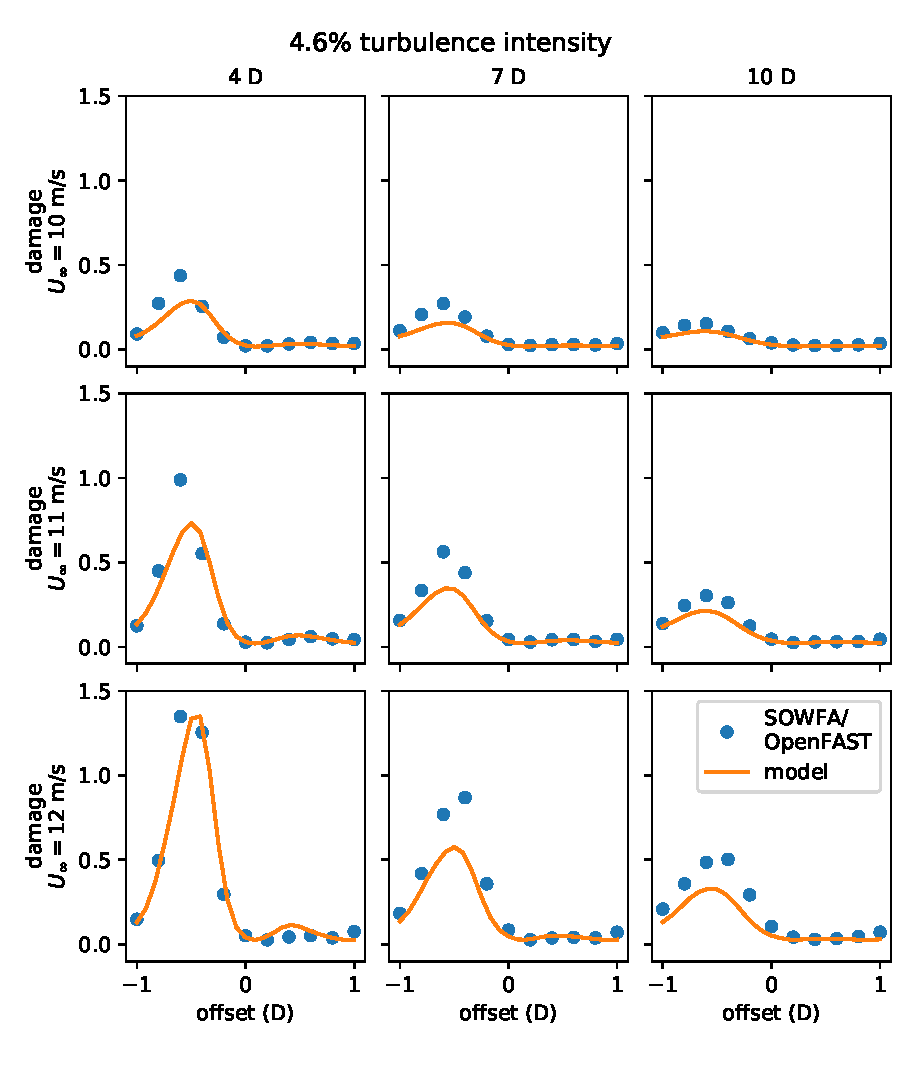
\includegraphics{images/lowTI_damage.pdf}
%     \caption{Comparison of our presented damage model to the damage predicted by the loads from the SOWFA and OpenFAST data. This figure is for a freestream turbulence intensity of 4.6\%. From top to bottom, each row represents different freestream wind speeds of 10, 11, and 12 meters per second. From left to right, each column represents different distances from the upstream turbine of 4, 7, and 10 rotor diameters.}
%     \label{low_TI}
% \end{figure}
% % 
% \begin{figure}
%     \centering
%     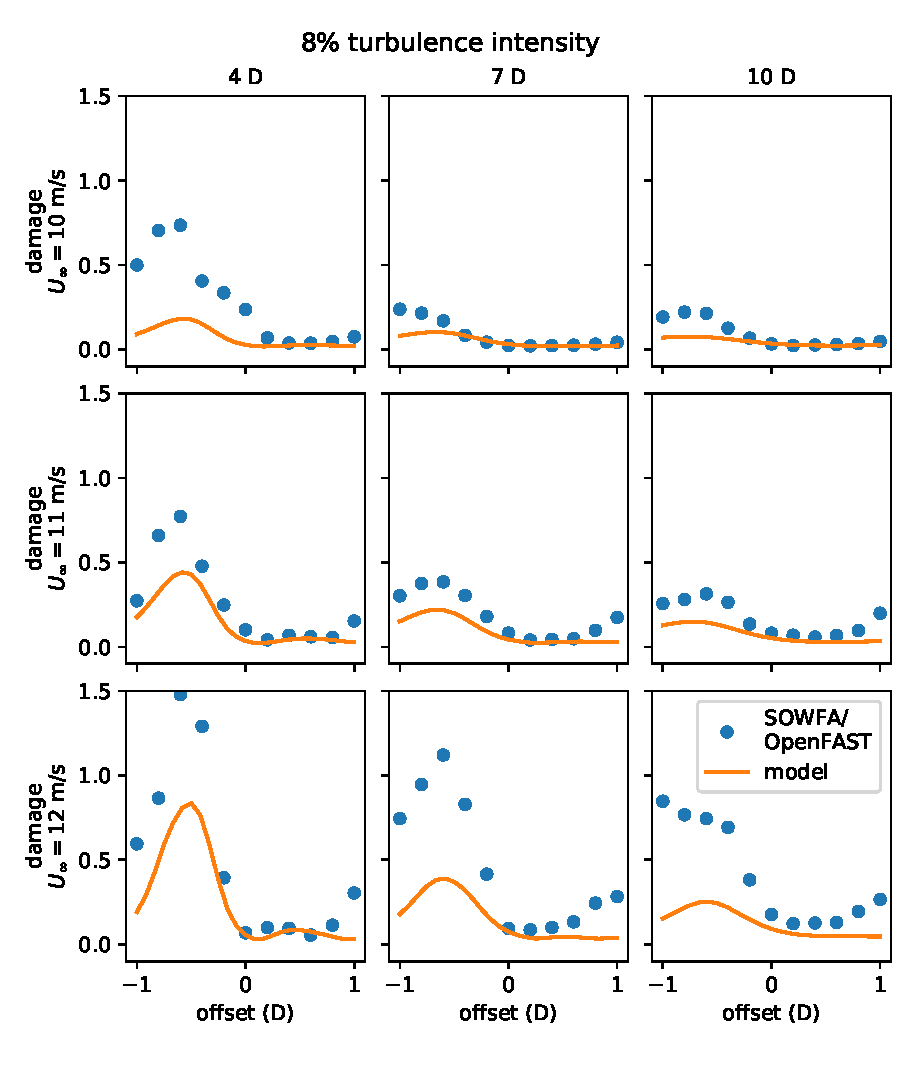
\includegraphics{images/highTI_damage.pdf}
%     \caption{Comparison of our presented damage model to the damage predicted by the loads from the SOWFA and OpenFAST data. This figure is for a freestream turbulence intensity of 8\%. From top to bottom, each row represents different freestream wind speeds of 10, 11, and 12 meters per second. From left to right, each column represents different distances from the upstream turbine of 4, 7, and 10 rotor diameters.}
%     \label{high_TI}
% \end{figure}
% % 
% 
\begin{figure}
    \centering
    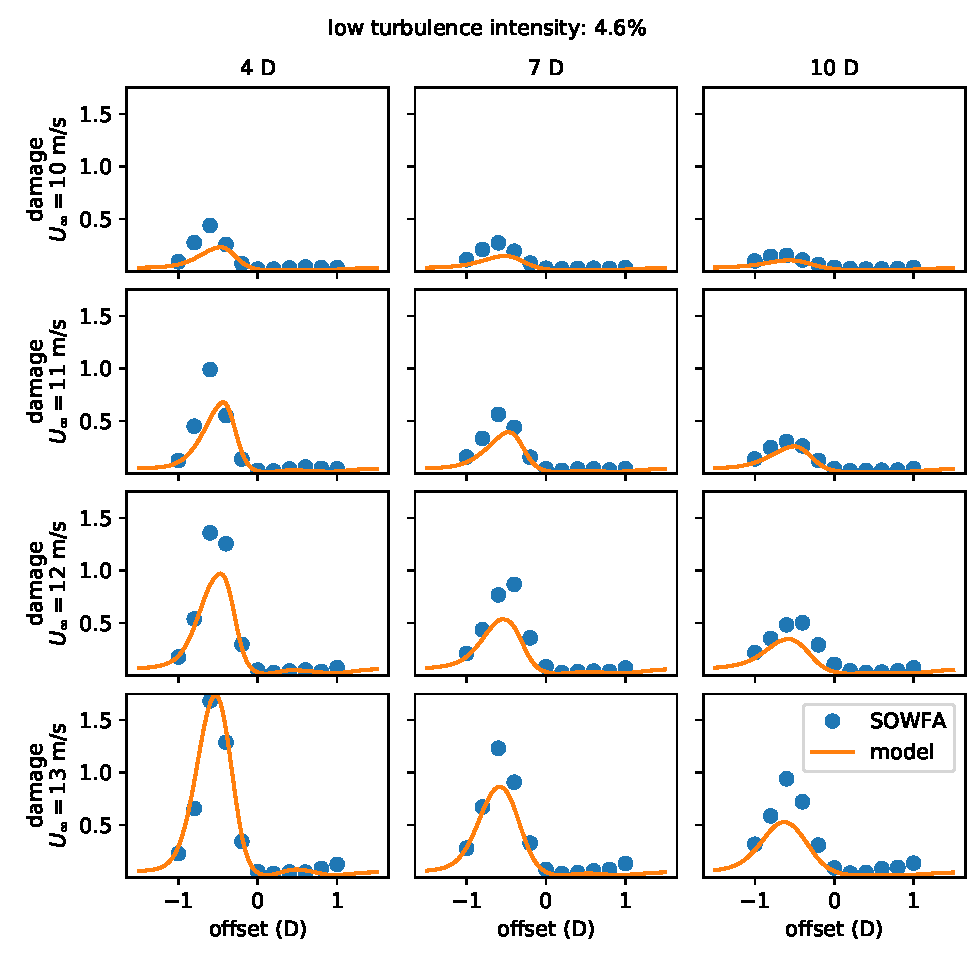
\includegraphics{images/damage_lowTI.pdf}
    \caption{Comparison of our presented damage model to the damage predicted by the loads from the SOWFA and OpenFAST data. This figure is for a low freestream turbulence intensity of 4.6\%. From top to bottom, each row represents different freestream wind speeds of 10, 11, 12 and 13 meters per second. From left to right, each column represents different distances from the upstream turbine of 4, 7, and 10 rotor diameters.}
    \label{low_TI}
\end{figure}
% 
\begin{figure}
    \centering
    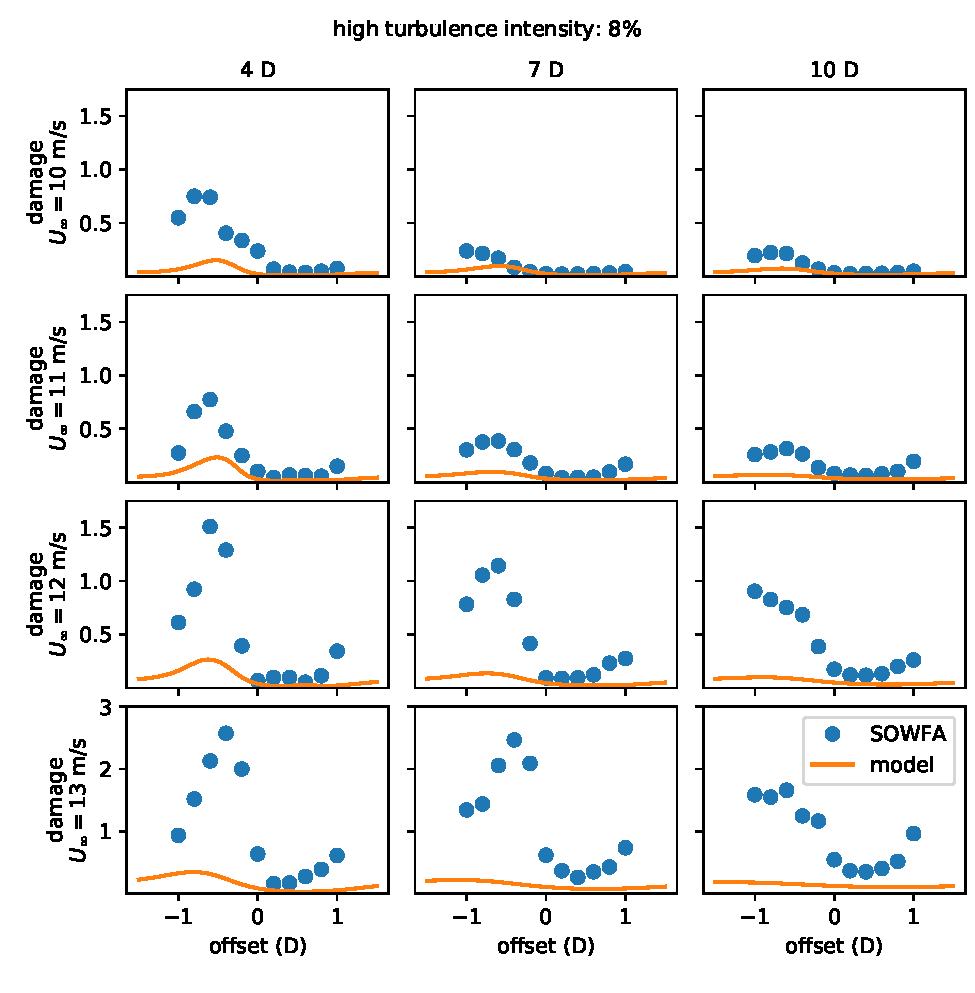
\includegraphics{images/damage_highTI.pdf}
    \caption{Comparison of our presented damage model to the damage predicted by the loads from the SOWFA and OpenFAST data. This figure is for a high freestream turbulence intensity of 8\%. From top to bottom, each row represents different freestream wind speeds of 10, 11, 12 and 13 meters per second. From left to right, each column represents different distances from the upstream turbine of 4, 7, and 10 rotor diameters.}
    \label{high_TI}
\end{figure}

The reason that the model performs so poorly in the high turbulence case is not an issue with the fatigue model itself, but is an issue with the other models on which the fatigue model is dependent. Referring back to Figs.~\ref{vels_highTI} and \ref{TI_highTI}, remember that the analytic wake and turbulence models we used were not good matches to the high fidelity SOWFA data. If we directly use the velocity and turbulence intensity profiles from SOWFA (the blue lines from Figs.~\ref{vels_highTI} and \ref{TI_highTI}) within our simple fatigue model, the damage prediction is much better. This comparison is shown in Fig.~\ref{SOWFA_damage}.
% 
\begin{figure}
    \centering
    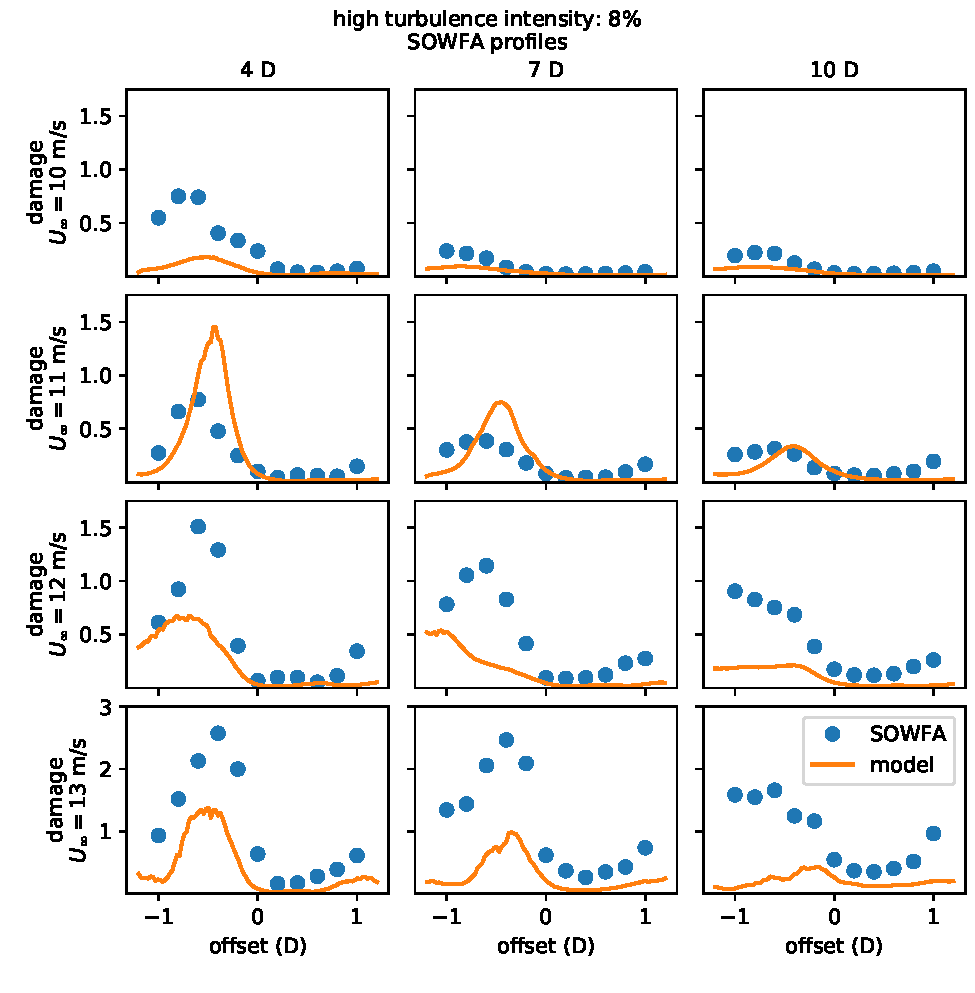
\includegraphics{images/damage_highTI_SOWFA.pdf}
    \caption{Comparison of our simple fatigue damage model using velocity and turbulence intensity profiles from SOWFA, to the damage predicted by the loads from the SOWFA and OpenFAST data. This figure is for a high freestream turbulence intensity of 8\%. From top to bottom, each row represents different freestream wind speeds of 10, 11, 12 and 13 meters per second. From left to right, each column represents different distances from the upstream turbine of 4, 7, and 10 rotor diameters.}
    \label{SOWFA_damage}
\end{figure}
% 
As with the low turbulence intensity case, the predicted damage from our model does not exactly match the higher fidelity damage prediction. However, when we run our model with the velocty and turbulence intensity profiles from SOWFA, we are able to achieve better comparison to the high fidelity data. This is important to remember, that the results from our presented fatigue damage model are fully dependent on the accuracy of the wake model and local turbulence intenstiy models being used.

% For wind speeds lower than those shown in Figs.~\ref{low_TI} and \ref{high_TI} (less than 10 meters per second), our model matches the SOWFA and OpenFAST data very well. However, with the current formulation of our model we are massively underpredicting the damage at higher wind speeds. Figure \ref{thirteen} shows the damage value comparisons for the low turbulence case and a wind speed of thirteen meters per second. As can be seen in this figure, our model is predicting very little damage, while the high fidelity data is still indicating that significant damage occurs for a partially waked turbine at this wind speed. This wind speed is above the rated wind speed for the wind turbine, and is high enough that even when the downstream is waked or partially waked it is above the rated wind speed. This means that, in theory, the blades would be pitched which would dramatically decrease the loading. While this is what our model predicts in the current formulation, the SOWFA and OpenFAST data for this scenario predicts lower pitch angles than we are in the model, which is at least partially responsible for large differences in the damage predictions. Because our model correctly predicts the locations and trends of turbine damage, the inaccuracies of our model in predicting the damage for the high turbulence and high wind speed cases do not render the model useless. It can still be used to identify and reduce areas of harmful partial waking. That said, improvements to the model to increase the accuracy of these scenarios would be beneficial.
% 
% \begin{figure}
%     \centering
%     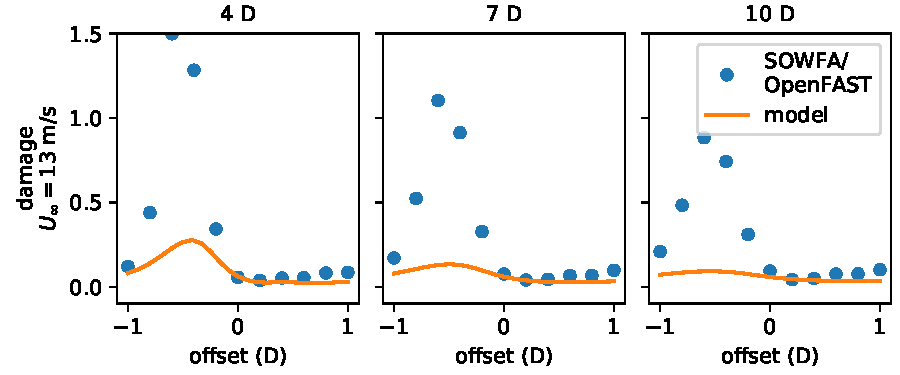
\includegraphics{images/damage_13.pdf}
%     \caption{Comparison of our presented damage model to the damage predicted by the loads from the SOWFA and OpenFAST data. This figure is for a freestream turbulence intensity of 4.6\% and a freestream wind speed of 13 meters per second. From left to right, each subfigure represents different distances from the upstream turbine of 4, 7, and 10 rotor diameters.}
%     \label{thirteen}
% \end{figure}

One observation that is consistent across all of the results shown in Figs.~\ref{low_TI}--\ref{SOWFA_damage} is that the fatigue damage is higher when the turbine is partially waked on one side (with a negative offset, in how we have presented the data), but the damage is slightly lower or at least unaffected when it is partially waked on the other side. While at first this may seem unintuitive, there is a simple explanation for this behavior caused by the interaction of the gravitational loads and the lead-lag aerodynamic loads. If the blade is partially waked while rotating upwards, the aerodynamic loads on the blade will be relatively lower. This means there is a smaller force to offset the gravitational loads, and the load fluctuations will be higher than if the turbine is operating in freestream conditions. On the other hand, if the blade is partially waked while rotating downwards, the aerodynamic loads acting in the same direction as the gravitational force are relatively lower. In this configuration, the load fluctuations are smaller than in freestream operating conditions. These interactions are explained more clearly in Fig.~\ref{partial_loading}.
% 
\begin{figure}
    \centering
    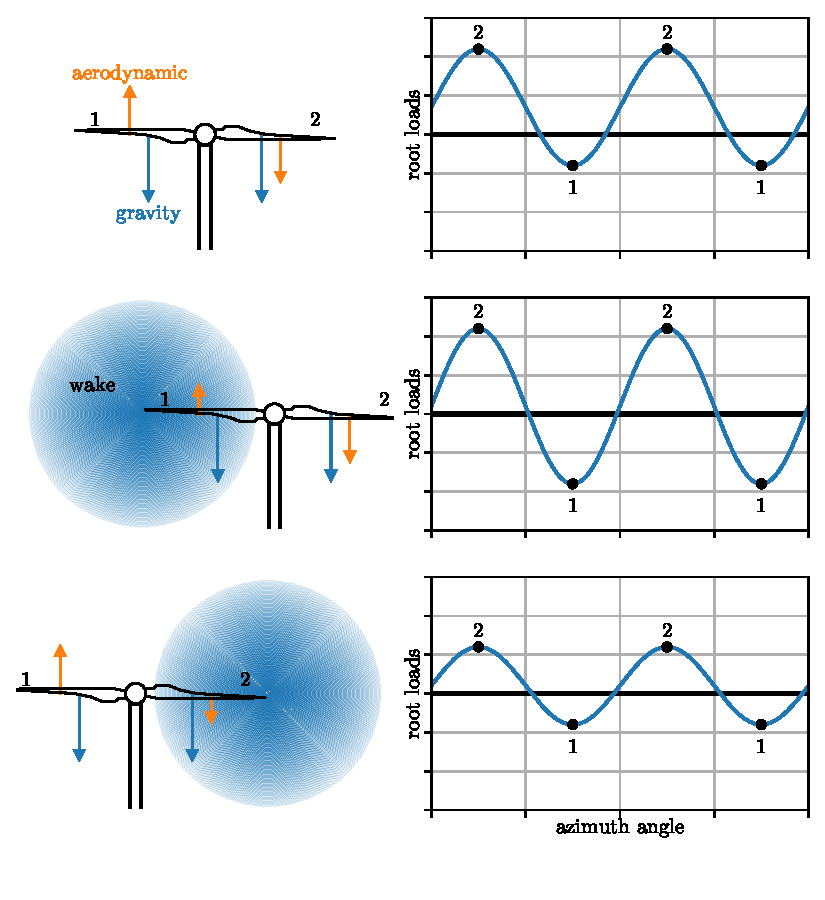
\includegraphics{images/partial_loading.pdf}
    \caption{Exaggerated lead-lag load differences for different waking scenarios. Shown conditions are freestream, partially waked that increase load fluctuations, and partially waked that decrease load fluctuations. The different combinations of the gravitational force and the aerodynamic force along the blade cause different load fluctuations. Blade positions 1 and 2 are labeled on the turbine figures on the left, which correspond to the numbered points in the loading figures on the right. }
    \label{partial_loading}
\end{figure}

\section{Example Optimization}

In this section we will discuss example wind farm layout optimizations in which we used our model to constrain the damage caused by partial waking throughout the wind farm. Before discussing the optimizations and the results, we'll briefly describe the models and assumptions we've made for these optimizations. As with the rest of this paper, these example optimizations assumed the NREL 5-MW reference turbine design throughout the farm. This turbine has a rotor diameter of 126.4 meters, a hub height of 90 meters, a cut-in wind speed of 3 meters per second, a rated wind speed of 11.4 meters per second, and a rated power of 5 megawatts. The power curve for this turbine was assumed to be perfectly cubic, as represented in Eq.~\ref{power_curve}. 
% 
\begin{equation}
    P = \begin{cases} 
      0 &  U_\text{eff} < U_\text{cut-in} \\
      (U_\text{eff}/U_\text{rated})^3 P_\text{rated} &  U_\text{cut-in} \leq U_\text{eff} < U_\text{rated}\\
      P_\text{rated} & U_\text{eff} \geq U_\text{rated}
   \end{cases}
   \label{power_curve}
\end{equation}
% 
In this equation, $U_\text{eff}$ is the effective inflow speed to the turbine, $U_\text{cut-in}$ is the cut-in wind speed, $U_\text{rated}$ is the rated wind speed, and $P_\text{rated}$ is the rated power.
We assumed wind speeds that were all relatively low, and thus did not need to consider a cut-out wind speed.
Additionally, we assumed the turbines always faced directly into the oncoming wind, that the terrain was flat, and a safety factor of 1.25 for the fatigue calculations.

Figure \ref{windrose} shows the wind rose and wind speed distributions we used for this study. This wind probability distribution is from the Horns Rev wind farm, as is the wind speed distribution, except we increased all of the wind speeds by three meters per second so they were closer to the rated wind speed of the NREL 5-MW reference turbine. We used 100 wind direction bins (every 3.6 degrees) in each optimization. Because the turbine fatigue is worst for partially waked orientations, it requires a large number of wind direction samples. We found 100 bins to be sufficient to appropriately approximate the damage. We assumed directionally averaged wind speeds, meaning we assumed the wind speed from each direction was always the mean wind speed from that direction. We assumed a wind shear exponent of 0.15, and a freestream turbulence intensity of 4.6\% (corresponding to Fig.~\ref{low_TI} for the damage calculations).
% 
\begin{figure}
    \centering
    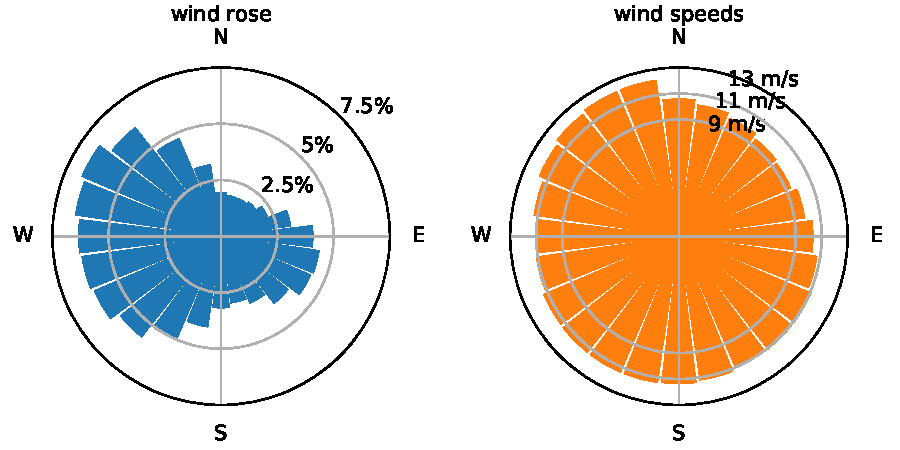
\includegraphics{images/windrose.pdf}
    \caption{The wind rose and directional wind speeds used in our optimization. The data is divided into 100 bins, one every 3.6 degrees.}
    \label{windrose}
\end{figure}

The objective of this optimization was to maximize the annual energy production (AEP) of the wind farm with respect to the location of each turbine. The rotor hubs were constrained to be at least two rotor diameters apart from each other. Additionally there were boundary constraints which forced the turbines to remain in a fixed wind farm boundary. Finally, the total fatigue damage was constrained to be less than a desired value. When considering fatigue damage, the assumption is that failure occurs when the damage value reaches unity. However, with the layout optimization we are only considering the additional damage caused by waking and partial waking of the wind turbines. Other significant drivers of fatigue are extreme wind gusts and cases of extreme wind shear and veer. These phenomena are not captured with our presented model, therefore we must constrain the optimization to some value less than one. In full, this optimization is represented in Eq.~\ref{optimization}.
% 
\begin{equation}
			\begin{aligned}
				& \text{maximize}
					& & \text{AEP} \\
                & \text{w.r.t.} 
                	&& x_j,~ y_j ~ (j = 1, \ldots, \text{nTurbs})\\
				& \text{subject to}
					& & \text{boundary constraints} \\
						&&& \text{spacing constraints} \\
						&&& \text{damage}_j < \text{damage}_\text{max} ~ (j = 1, \ldots, \text{nTurbs})
			\end{aligned}
		\label{optimization}
		\end{equation}

We used the optimizer SNOPT for these examples, which is a gradient-based optimizer which works well for large problems with many design variables and constraints \cite{gill2005snopt}. We provided exact, analytic gradients to the optimizer using ForwardDiff, an automatic differentiation package in Julia \cite{revels2016forward}.
In order to provide a point of reference and find a starting point for our final optimization with damage constraints, we first ran 50 optimizations of the wind farm without damage constraints and with randomly initialized design variables. We then chose the layout with the highest AEP, and used that as the starting point for our optimizations with loads constraints.


\subsection{Example Optimization 1}

The first example optimization we performed was for a wind farm with 40 wind turbines and with an parallelogram shaped boundary. The average turbine spacing for this wind farm was 6 rotor diameters. The damage was constrained to be less than 0.16, which is about a 40\% reduction from the maximum damage for the optimized layout without damage constraints.
Figures \ref{layouts} and \ref{opt_damages} show the results from this example optimization. Figure \ref{layouts} shows the optimal turbine layouts with and without damage constraints. The AEP for the turbine layout without damage constraints is 1159 GWh, while the AEP for the layout with damage constraints is 1150 GWh. With the optimization method we used, there is a small sacrifice in AEP of less than 1\% required to meet the damage constraints. Notice the small differences in the layouts with and without damage constraints. 
While small variations can be seen throughout the wind farm, the most visible differences are seen on the left and right boundaries, where the turbines are spaced very close together. Looking at Fig.~\ref{low_TI}, we can see that the damage from partial waking can be very high when the turbines are close together. Therefore, in order to meet the damage constraints, these turbines that started close together needed to be carefully repositioned in order to avoid configurations with detrimental partial waking. Turbines that were already spaced far apart did not need to move as much because the wakes between these turbines already recovered most of the way, meaning damage from partial waking is already minimal.
% 
\begin{figure}
    \centering
    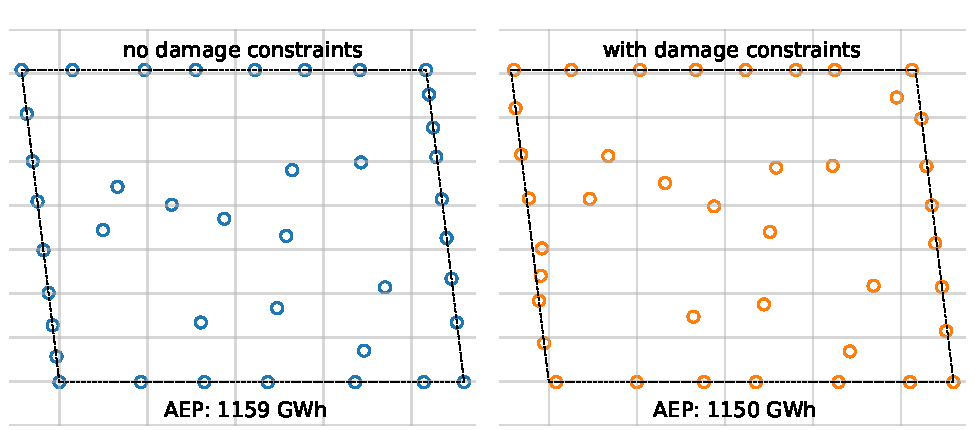
\includegraphics{images/opt_layouts40.pdf}
    \caption{The optimal layout results from our optimization. On the left are the optimal turbine locations when the turbine layout is optimized without damage constraints. On the right are the turbine locations when damage from partial waking is constrained to be less than 0.16. The dotted black lines represent the wind farm boundary, and the circles represent the wind turbines, with the circle diameter accurately scaled to represent the turbine rotor diameter.}
    \label{layouts}
\end{figure}


Figure \ref{opt_damages} shows the total damage accumulated by every turbine for each of the layouts shown in Fig.~\ref{layouts}. For the layout which was optimized without damage constraints, a little less than half of the turbines violate the desired maximum damage of 0.16, with the highest individual turbine damage near 0.25. With damage constraints activated, we were able to reduce the damage from partial waking to the desired value for every turbine in the wind farm, including the ones with a very high initial damage values near 0.25.
% 
\begin{figure}
    \centering
    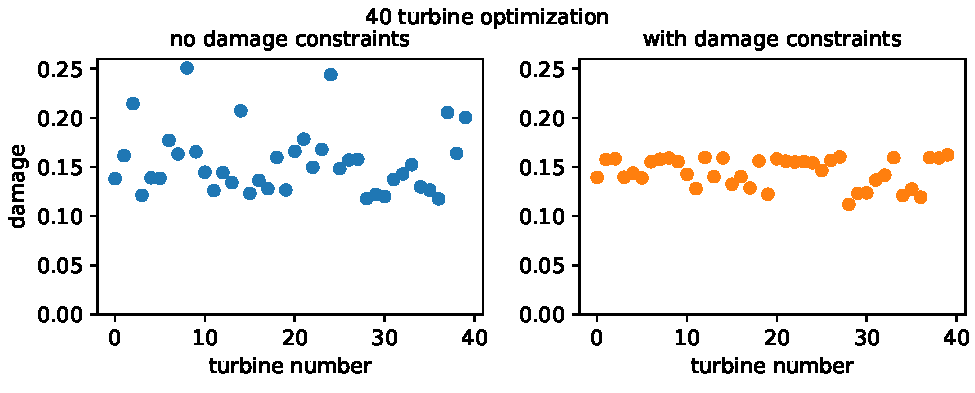
\includegraphics{images/opt_damage_vals40.pdf}
    \caption{The fatigue damage of each turbine in our wind farm layout optimizations. On the left are the damages for the wind farm layout optimized without damage constraints, while on the right are the damages with the maximum damaged constrained to be less than 0.16.}
    \label{opt_damages}
\end{figure}




\subsection{Example Optimization 2}

The second example optimization we performed was for a wind farm with 20 wind turbines and a circular boundary. The average turbine spacing for this wind farm was 4 rotor diameters, meaning the turbines in this farm were, on average, very close together. The damage was constrained to be less than 0.215, which is about a 30\% reduction from the maximum damage for the optimized layout without damage constraints.
Figures \ref{layouts_circ} and \ref{opt_damages_circ} show the results from this second example optimization. As with the results for the first example optimization, Fig.~\ref{layouts_circ} shows the optimal turbine layouts with and without damage constraints. The AEP for the turbine layout without damage constraints is 538.8 GWh, while the AEP for the layout with damage constraints is 532.0 GWh, indicating that the AEP reduced by just over 1\% in order to constrain the damage to the desired value. 
Because the wind turbines in this farm are spaced much closer together than those in the first example optimization, as a whole the turbines moved more in order to meet the damage constraints. Again, the largest differences are experienced by the turbines near or on the boundary, which are spaced close together. Partial waking when the turbines are that close together creates large load fluctuations, and is therefore extremely detrimental from a fatigue damage perspective.


% Notice the small differences in the layouts with and without damage constraints. While small variations can be seen throughout the wind farm, the most visible differences are seen on the left and right boundaries, where the turbines are spaced very close together. Looking at Fig.~\ref{low_TI}, we can see that the damage from partial waking can be very high when the turbines are very close together. Therefore, in order to meet the damage constraints, these turbines that started close together needed to be carefully repositioned in order to avoid configurations with detrimental partial waking. Turbines that were already spaced far apart did not need to move as much because the wakes between these turbines already recovered most of the way, meaning damage from partial waking is already minimal.
% 
\begin{figure}
    \centering
    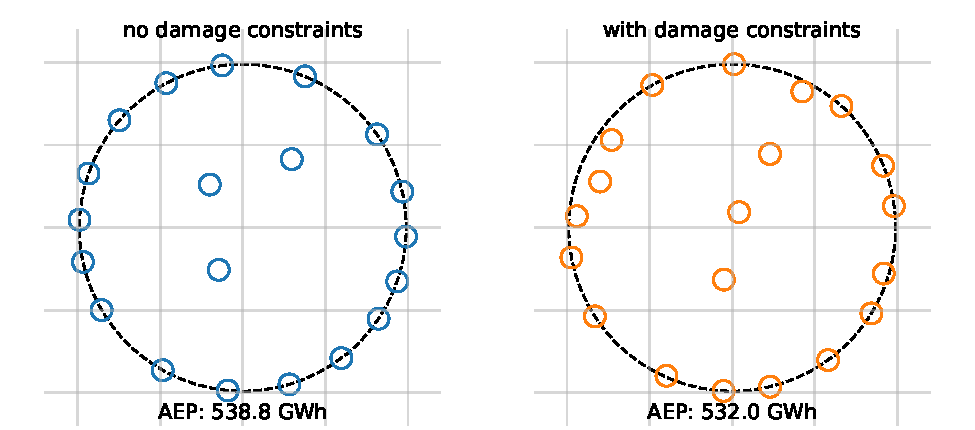
\includegraphics{images/opt_layouts20.pdf}
    \caption{The optimal layout results from our optimization. On the left are the optimal turbine locations when the turbine layout is optimized without damage constraints. On the right are the turbine locations when damage from partial waking is constrained to be less than 0.215. The dotted black lines represent the wind farm boundary, and the circles represent the wind turbines, with the circle diameter accurately scaled to represent the turbine rotor diameter.}
    \label{layouts_circ}
\end{figure}


Figure \ref{opt_damages_circ} shows the total damage accumulated by every turbine for each of the layouts shown in Fig.~\ref{layouts_circ}. As with example optimization one, a little less than half of the turbines had higher than the desired damage values when the layout was optimized without damage constraints. When the damage from partial waking was constrained, the optimization successfully limited every turbine damage below the desired value of 0.215.
% For the layout which was optimized without damage constraints, a little less than half of the turbines violate the desired maximum damage of 0.16, with the highest individual turbine damage near 0.25. With damage constraints activated, we were able to reduce the damage from partial waking to the desired value for every turbine in the wind farm, including the ones with a very high damage values near 0.25.
% 
\begin{figure}
    \centering
    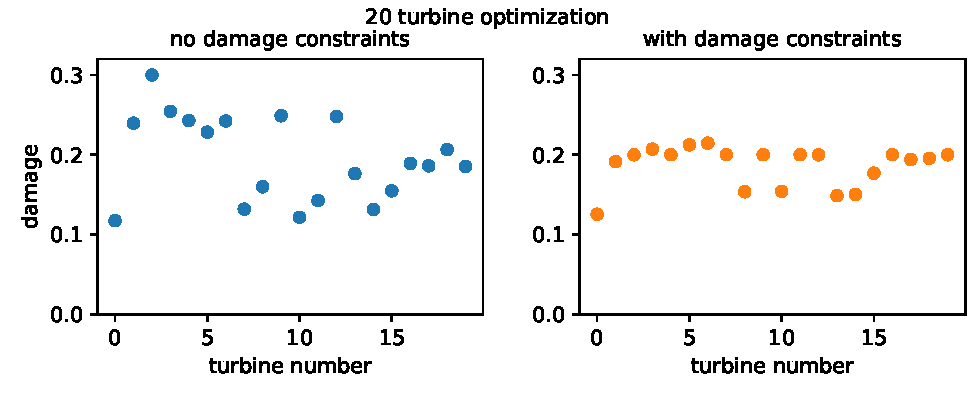
\includegraphics{images/opt_damage_vals20.pdf}
    \caption{The fatigue damage of each turbine in our wind farm layout optimizations. On the left are the damages for the wind farm layout optimized without damage constraints, while on the right are the damages with the maximum damaged constrained to be less than 0.215.}
    \label{opt_damages_circ}
\end{figure}



\subsection{Multi-objective Optimization}

The example optimizations discussed above assumed we have prior knowledge of the desired maximum damage value for turbines in the wind farm, which may not always be the case. Often, one may want to both maximize the energy production of the wind farm, while also minimizing the damage accumulated by each of the turbines in order to extend their lifetimes. To demonstrate this scenario, we used the epsilon-constraint method to create a Pareto front of the maximum AEP and maximum turbine damage for each of the example optimizations we discussed. Multi-objective optimization using the epsilon-constraint method is performed by repeatedly optimizing and objective, in our case to maximize the AEP, with successively stricter constraints, which in our case means to decrease the maximum allowable turbine damage. Figure \ref{pareto} shows the Pareto fronts from these optimizations. In this figure, the AEP on the y-axis has been normalized by the maximum AEP obtained when the layout is optimized without any damage constraints. 
% 
\begin{figure}
    \centering
    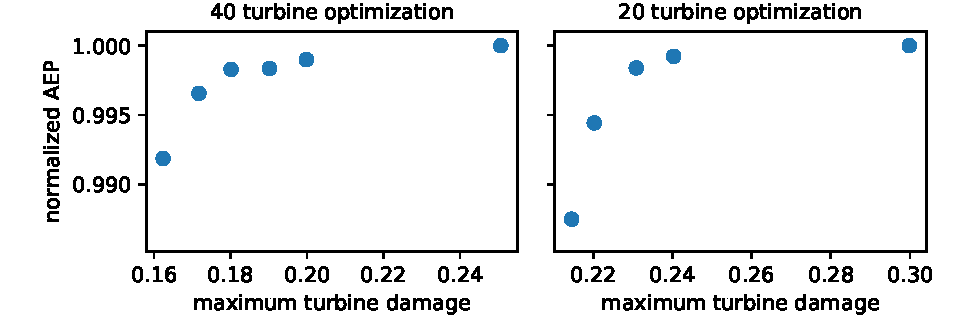
\includegraphics{images/damage_aep_paretos.pdf}
    \caption{Pareto fronts displaying the trade-offs  between maximizing AEP and minimizing turbine damage. The y-axis for these figures has been normalized by the maximum AEP achieved without constraining the turbine damage.}
    \label{pareto}
\end{figure}

There are three main observations that we can take away from these Pareto fronts. First, there is a large flat area in the Paerto front, which indicates that we can constrain the maximum damage by a significant amount with very little impact to the AEP. For the 40-turbine wind farm, the damage can be constraint to 0.18, with a very small AEP reduction of 0.1--0.2\%. For the 20-turbine wind farm, the damage can be constrained to a value of 0.23, again with a very small reduction in the AEP. The damage can be significantly constrained practically for free. 
% 
Second, The most strict damage constraint for each wind farm can be achieved with a small impact on the AEP. A 1\% reduction in AEP is certainly not negligible, however it is noteworthy that the most strict constraint on the turbine damage can be applied with such a small reduction in AEP. As has been discussed in detail, partial waking can greatly increase the fatigue damage on a wind turbine. In addition to increasing damage, partial waking is also detrimental from a power production perspective, as any amount of waking decreases the effective wind speed and therefore the power produced by a turbine. Therefore, an optimal wind farm layout that maximizes AEP will aim to reduce any waking as much as possible. This means that a wind farm optimized to maximize energy production, and a wind farm optimized to minimize turbine damage share many similarities. Each objective can achieve a desirable value without forcing a significant trade-off from the other.
% 
Lastly, we can see from these Pareto fronts that the 40-turbine wind farm with an average turbine spacing of 6 rotor diameters has lower turbine damages than the 20-turbine wind farm with an average spacing of 4 rotor diameters. The wind farm with large average spacing between turbines has more space to move the turbines, and can find layouts which produce large amounts on energy in addition to lower damages. Also, when the turbines are spaced farther apart, the wake impacts are not as severe. This means that the load fluctuations, and therefore the fatigue damage are also not as large when the turbines are far apart. The opposite is true of the more dense wind farm. When the turbines are close together, the damage values are higher, and cannot be constrained to very low values.






\section{Conclusions}
In this paper, we have presented a model to predict fatigue damage on wind turbines caused by partial waking throughout the farm. The model predicts the trends of turbine damage very well, and the configurations with the worst damage. The model we presented is computationally efficient, such that is can be used in an optimization framework to constrain or minimize the turbine damage throughout the wind farm. We demonstrated using the model in example optimizations, in which we optimized the layout of turbines in a wind farm while constraining the damage caused by partial waking. We found that, at least in the cases that we explored, the damage could be successfully reduced by 30-40\% with a sacrifice to the optimal annual energy production around 1\%. Additionally we performed a multi-objective optimization, which shows that if we allow the maximum turbine damage to be slightly higher, the damage can be constrained with negligible sacrifice to the AEP of 0.1--0.2\%.

The area of loads and fatigue consideration in wind farm layout optimization has huge potential for continued research. For continuation of this research paper, we have a few specific recommendations. 
% 
First, improve the intermediate wind speed and local turbulence intensity models for high turbulence cases.  Figures \ref{low_TI} and \ref{high_TI} show that the current models predict trends and actual damage values very well for low turbulence conditions. For high turbulence conditions, the models predict the trends well but severely underpredict the damage values. 
% 
Second, conduct a deeper investigation into how including damage constraints in wind farm layout optimization affects farm design and performance. For the example optimizations we have shown, and in simple optimizations we have run in the past \cite{stanley2020wind}, we found that the damage can be constrained with minimal sacrifice to the energy production. Considering a wider variety of wind farms and wind resources would be useful to confirm or clarify this conclusion.
% 
Third, we recommend coupling our proposed model with active wind farm control optimization. Additional damage reductions are likely achievable by coupling layout and control optimization. Using active yaw control for wake steering would be particularly interesting with fatigue damage constraints. As we demonstrated in this paper, the partial waking is detrimental for fatigue damage on one side of the turbine, and negligible or significantly lower on the other side. Wake steering through yaw control gives the freedom to deflect wakes in either direction behind a wind turbine, which could increase power production by partially waking downstream turbines on the side that does not increase fatigue damage.

Recent years have seen significant improvements in wind energy technology, and large reductions in the cost to produce wind energy.
The model that we have proposed is an additional improvement, allowing wind farm layout optimization which considers turbine loading and fatigue, which will further decrease the cost of wind energy. %By considering turbine fatigue damage during layout optimization, wind turbines can have an extended lifetime.
% Current research includes using active turbine control to reduce loading on turbines, including more research into turbine de-rating as wind farms begin to reach the end of their original design lifetime. 
% These areas will continue to be important areas of focus, however fatigue damage will be further reduced when considered during layout optimization of the wind farm.

\section*{Code and data availability}
With the exception of the optimizer SNOPT, all of the code and models used in this study are open source. The wind farm models, optimization framework, and damage model are available here: \url{https://github.com/byuflowlab/FlowFarm.jl}. The individual run scripts and plot generation scripts are available here: \url{https://github.com/pjstanle/loads-journal}.

\section*{Author Contributions}


\section*{Competing Interests}
The authors declare no competing interests.

\section*{Acknowledgements}

\FloatBarrier
\bibliographystyle{unsrt}
\bibliography{references.bib}

\section*{Appendix 1: Large Eddy Simulation}
\label{sec:les}

We used Simulator fOr Wind Farm Applications (SOWFA) to generate the inflow data which we then used to calculate the loads with which to compare our model.  SOWFA is a high-fidelity large eddy simulation tool that was developed at the National Renewable Energy Laboratory for wind farm studies.  It is based on the open source CFD solver OpenFOAM, and can be coupled with NREL's FAST modeling tool.  SOWFA has been used in several previous wind farm control studies \cite{fleming2013sowfa,fleming2015simulation,gebraad2016wind}.  

In this paper, SOWFA uses an actutator disk model to represent the turbine in an atmospheric boundary layer.  It solves the three-dimensional incompressible Navier-Stokes equations and transport of potential temperature equations, which take into account thermal buoyancy and Earth rotation (Coriolis) effects in the atmosphere.  The inflow conditions for this simulation are generated using a periodic atmospheric boundary layer precursor with no turbines.  Additional details can be found in \cite{fleming2013sowfa}. 

All simulations performed in this study used a neutral boundary layer and were simulated in a 5km$\times$2km$\times$1km domain.  Low turbulence cases had approximately 4.6$\%$ turbulence intensity and high turbulence cases has approximately 8$\%$ turbulence intensity.  Simulations were run for the following cases:
\begin{itemize}
    % \item 6\,m/s low and high turbulence
    % \item 8\,m/s low and high turbulence
    % \item 9\,m/s low and high turbulence
    \item 10\,m/s low and high turbulence
    \item 11\,m/s low and high turbulence
    \item 12\,m/s low and high turbulence
    \item 13\,m/s low and high turbulence
    % \item 18\,m/s high turbulence in a 3km$\times$3km domain
\end{itemize}

Inflow data for the OpenFAST simulations was generated based on the respective SOWFA simulations for the different cases. Slices of the SOWFA data were taken at different distances downstream from an upstream turbine, as shown in Figure~\ref{fig:sowfa_slices_for_FAST_input}. These planes were then processed from the SOWFA .vtk data into three component wind files (U, V, and W) of the binary HAWC-style full-field format, which can be specified in the InflowWind.dat file used by OpenFAST. This process provided the time-series wind inflow information used by OpenFAST to generate the turbine load data at the different distances downstream, and at different cross stream locations.

\begin{figure}
    \centering
    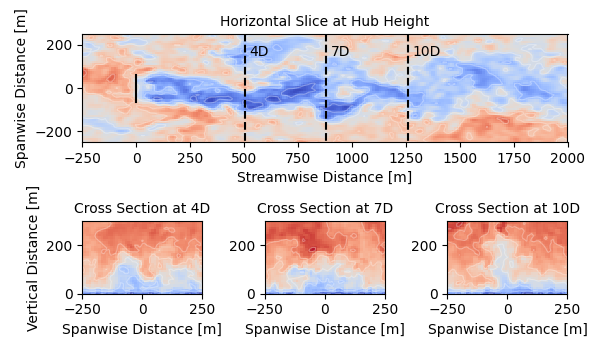
\includegraphics{images/sowfa_slices.png}
    \caption{Examples of SOWFA data used to generate inflow for FAST simulations.}
    \label{fig:sowfa_slices_for_FAST_input}
\end{figure}



\end{document}